\chapter{Theoretical Background}
\label{chap:Theory}
Since 1930s, many theories and discoveries in particle physics have revealed the fundamental structure of matter. The matter is made up of fundamental particles and their interactions are mediated by four fundamental forces \cite{Griffiths:111880}. The theoretical models describe all the phenomena of particle physics as well as predict the properties of particles. These models must be either confirmed experimentally or totally excluded giving hints of new physics. This interplay between experimental discoveries and the corresponding theoretical predictions leads to a theoretical model called Standard Model, which describes the fundamental particles and their interactions. The world's most powerful particle accelerators and detectors are used by physicists to test the predictions and limits of the Standard Model where it has successfully explained almost all experimental results. This chapter describes the Standard Model with main focus on the theory of strong interactions called Quantum Chromodynamics and its features which serve as the theoretical base of this thesis.

%The growing knowledge about fundamental and new particles was accompanied by the evolution of quantum mechanics and the special relativity. 
\section{Standard Model}
The Standard Model (SM) of particle physics \cite{Perkins:1982xb,Herrero:1998eq,Weinberg:1967tq} was developed in 1970s. It is a mathematical framework which describes the nature and properties of the fundamental particles and the three of the four known forces of interactions between them, as summarized in Fig.~\ref{fig:SM}. According to the SM, there are 12 elementary particles i.e. without any internal structure, known as fermions. The fermions have half integral spin and obey Fermi-Dirac statistics. They follow the Pauli exclusion principle according to which two or identical fermions cannot occupy the same quantum state. Each fermion has an associated anti-particle having the same properties but opposite-sign quantum numbers.
\begin{figure}[!h]
\begin{center}
\hspace*{-15mm}
%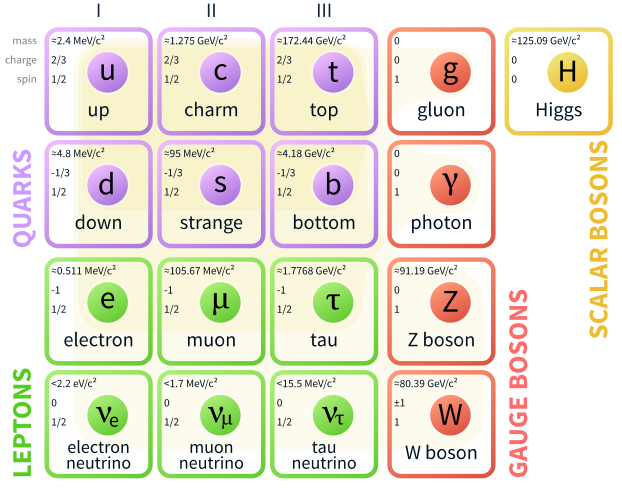
\includegraphics[scale = 0.8]{/home/anter/Desktop/Thesis/Figures/StandardModel_edited.png}\\
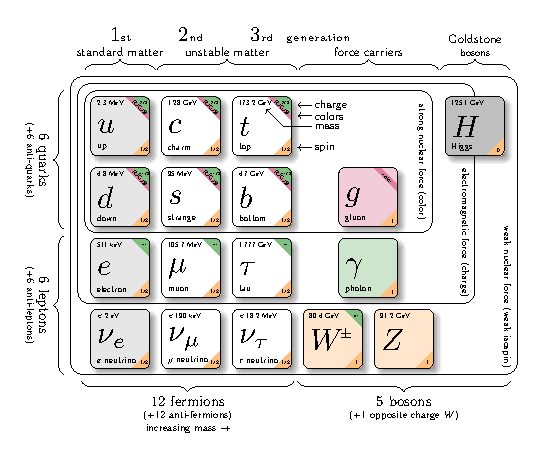
\includegraphics[width=1.2\textwidth]{/home/anter/Desktop/Thesis/Figures/model-physics.pdf}\\
%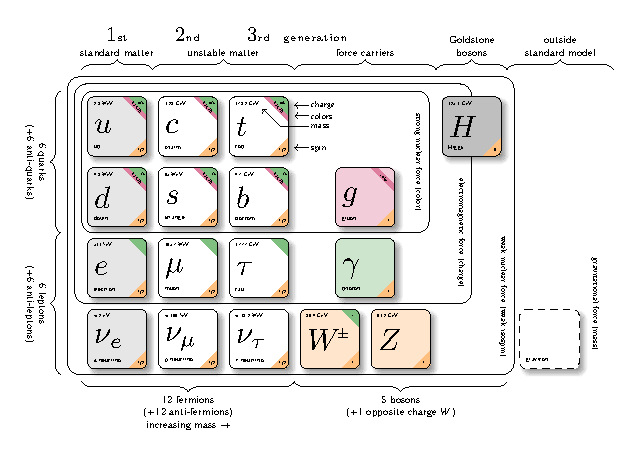
\includegraphics[width=1.2\textwidth]{/home/anter/Desktop/Thesis/Figures/original_model-physics.pdf}\\
\caption[The Standard Model summarizing the properties of elementary particles and their forces of interaction.]{The Standard Model\footnotemark summarizing the properties of elementary particles known as fermions (leptons and quarks) grouped into three generations, gauge bosons as mediators for the interactions, the scalar Higgs boson and not corporated graviton for the gravitational force.}
\label{fig:SM}
\end{center}
\end{figure}
\footnotetext{Source : \url{http://www.texample.net/tikz/examples/model-physics}}%https://en.wikipedia.org/wiki/Standard_Model}}
Depending on how the fermions interact, these are classified into two categories - leptons (\sln) and quarks ($q$). The leptons are of six types : electron ($e$), muon ($\mu$) and tau ($\tau$) with electric charge Q = -1\footnote{all charges are expressed in units of elementary charge $e$} and the corresponding neutrinos : electron neutrino ($\nu_e$), muon neutrino ($\nu_\mu$) and tau neutrino ($\nu_\tau$) having electric charge Q = 0. The quarks exist in six ``flavors'' : up ($u$), down ($d$), strange ($s$), charm ($c$), bottom ($b$) and top ($t$). $u$, $c$ and $t$ carry electric charge Q = $\pm$ $\frac{2}{3}$ whereas $d$, $s$ and $b$ carry Q = $\pm$ $\frac{1}{3}$. The quarks and leptons are categorized into three generations. The first generation has the lightest and the most stable particles whereas the heavier and less stable particles belong to the second and third generations.

The four fundamental forces exist in nature : electromagnetic, strong, weak and gravitational force. Every interaction involves the exchange of a gauge boson : the photon ($\gamma$) for the electromagnetic force, gluons ($g$) for the strong force, two $W$'s and a $Z$ for the weak force and the graviton (not yet found) for the gravitational force. However, the gravitational force has not been incorporated into SM yet. Along with this, the existence of dark matter or dark energy and the matter-antimatter asymmetry are still missing pieces in the SM. The interaction between fundamental particles acts because of some peculiar property of the particles - charge for the electromagnetic force, color for the strong force and flavor for the weak force. 

In the SM, the first three forces are unified into one quantum field theory \cite{Peskin:1995ev}, known as Grand Unified Theory (GUT) \cite{Glashow:1979pj,Salam:1980jd,Georgi:1974sy}. The SM framework based on quantum field theories is described by SU(3)$_{\rm C}~\otimes$ SU(2)$_{\rm L}~\otimes$ U(1)$_{\rm Y}$ gauge symmetry where C stands for the color charge, L for weak isospin and Y for hypercharge. Here SU(3)$_{\rm C}$, SU(2)$_{\rm L}$ and U(1)$_{\rm Y}$ terms give rise to strong, weak and electromagnetic forces, respectively. U($n$) are the unitary and SU($n$) are the special unitary groups of degree $n$ . The electromagnetic interaction of particles is explained by a well established modern theory called Quantum Electrodynamics (QED). In SM, the weak and electromagnetic interactions are combined by an electroweak theory. The spontaneous symmetry is broken due to the coupling to the scalar Higgs field which results in the massive $W^{\pm}$ and $Z$ bosons and the massless photon ($\gamma$). The Higgs boson, named after Peter Higgs, is the field quantum of the Higgs field responsible for electroweak symmetry breaking. Its existence was confirmed by the CMS \cite{Chatrchyan:2012xdj} and ATLAS \cite{Aad:2012tfa} collaborations in 2012, with the properties consistent with the SM. The SU(3)$_{\rm C}$ term defines the strong interaction between quarks and gluons mediated by gluons, with the three degrees of freedom of the color charge (C). In contrast to the electroweak symmetry, the SU(3)$_{\rm C}$ of the strong interaction is an exact symmetry and hence the gluons are massless. The strong interaction between quarks and gluons is described by theory called Quantum Chromodynamics (QCD), explained in details in the next section of this thesis.
%The gauge bosons of the unified electroweak theory are a mixture of the gauge bosons of the unbroken symmetry
\section{Quantum Chromodynamics}
The strong interactions between the quarks and gluons are described by a non-abelian gauge theory called Quantum Chromodynamics (QCD) \cite{Ellis:1991qj, Halzen:1984mc}. The gauge group of QCD is the special unitary group SU(3)$_{\rm C}$ with color charges C as the generators of the gauge group. Color charge is the peculiar property of QCD and has a same role as the electric charge in electromagnetic interactions. However, the mediator of electromagnetic interactions i.e. photon, itself does not carry any electric charge whereas the gluon itself carry color charge. This allows the self coupling of gluons and hence make the theory non-abelian. Both the quarks and gluons carry three types of color charges : red ($r$), green ($g$) and blue ($b$), and three types of anti-color charges : anti-red ($\bar{r}$), anti-green ($\bar{g}$) and anti-blue ($\bar{b}$). The quarks carry a single color charge whereas gluons carry a combination of color charges. There are nine eigen states of gluons but one of them $\frac{1}{\sqrt{3}}(r\bar{r}~\plus g\bar{g}~\plus b\bar{b})$ is totally symmetric color singlet which has no net color charge and does not take part in interaction. The remaining eight eigen states of the gluons are :
\begin{equation}
r\bar{b},~r\bar{g},~g\bar{r},~g\bar{b},~b\bar{g},~b\bar{r},~\frac{1}{\sqrt{2}}(r\bar{r}~-~b\bar{b}),~\frac{1}{\sqrt{6}}(r\bar{r}~\plus b\bar{b}~-~2g\bar{g}) 
\end{equation}

The dynamics of the quarks and gluons are controlled by the gauge invariant QCD Lagrangian $\mathcal{L}_{QCD}$ which is composed of four terms as : 
\begin{equation}
\mathcal{L}_{QCD} = \underbrace{-\frac{1}{4}F^A_{\mu\nu}F^{\mu\nu}_A}_\text{$\mathcal{L}_{gluons}$}~\plus \underbrace{\sum\limits_{flavors}^{} \bar{q}_a \big(i\gamma^\mu (D_\mu)_{ab}~-~m_q\big)q_b}_\text{$\mathcal{L}_{quarks}$}~\plus \mathcal{L}_{gauge}~\plus\mathcal{L}_{ghost}
\label{eq:lag}
\end{equation}
where $\mathcal{L}_{gluons}$ describes the kinetic term of the gluon fields ${\cal A}^A_\mu$; $\mathcal{L}_{quarks}$ defines the interaction between spin-$\frac{1}{2}$ quark fields $q_a$ of mass $m_q$ and spin-1 gluon fields ${\cal A}^A_\mu$ summing over all presently known six flavors of quarks; $\mathcal{L}_{gauge}$ describes the chosen gauge and $\mathcal{L}_{ghost}$ is the so-called ghost term required to treat the degeneracy of equivalent gauge field configurations in non-abelian gauge theories. In Eq.~\ref{eq:lag}, the Greek letters $\mu$, $\nu$, ... $\in$ \{0,1,2,3\} are the space-time indices; a,b,c $\in$ \{1,2,3\} and A,B,C $\in$ \{1,...,8\} are the indices of the triplet and octet representations, respectively, of the gauge symmetry group SU(3)$_{\rm C}$. The field tensor $F^A_{\mu\nu}$ is defined as
\begin{equation}
F^A_{\mu\nu} = \partial_\mu {\cal A}^A_\nu - \partial_\nu {\cal A}^A_\mu - g_s f_{ABC}{\cal A}^B_\mu {\cal A}^C_\nu
\label{eq:field}
\end{equation}
where $g_s$ is the coupling constant determining the strength of the interaction between colored partons and $f_{ABC}$ are the structure constants of the SU(3)$_{\rm C}$ group. The last term in Eq.~\ref{eq:field} is a non-abelian term which distinguishes QCD from QED and gives rise to a three- and a four-gluon vertex. In the term $\mathcal{L}_{quarks}$, ($D_\mu$)$_{ab}$ is the covariant derivative given by Eq.~\ref{eq:cov} and $\gamma_\mu$ are the Dirac $\gamma$-matrices. 
%In the second term of Eq.~\ref{eq:lag}, 
\begin{equation}
(D_\mu)_{ab} = \partial_{\mu}\delta_{ab}~\plus ig_sT^A_{ab}{\cal A}^A_\mu
\label{eq:cov}
\end{equation}
${\cal A}^A_\mu$ are the gluon fields with factors $T^A_{ab}$ factors corresponding to the generators of the SU(3)$_{\rm C}$ gauge group. The generators are represented via $T^A$ = $\lambda^A$/2 by the Hermitian and traceless Gell-Mann matrices $\lambda^A$ \cite{GellMann:1962xb}. The generator matrices $T^A$ follow the commutation relations :
\begin{equation}
\bigg[T^A,T^B\bigg] = if_{ABC}T^C
\end{equation}

In $\mathcal{L}_{QCD}$, the classical contribution comes from $\mathcal{L}_{gluons}$ and $\mathcal{L}_{quarks}$ terms which give rise to the free quark- and gluon-field terms, and the quark-gluon interaction terms presented in Fig.~\ref{fig:feyn}. The cubic and quartic gluon self-interaction vertices proportional to $g_s$ and $g^2_s$, respectively, come into play due to the non-abelian property of QCD.

\begin{figure}[!h]
\begin{center}
\hspace*{-1.3mm}

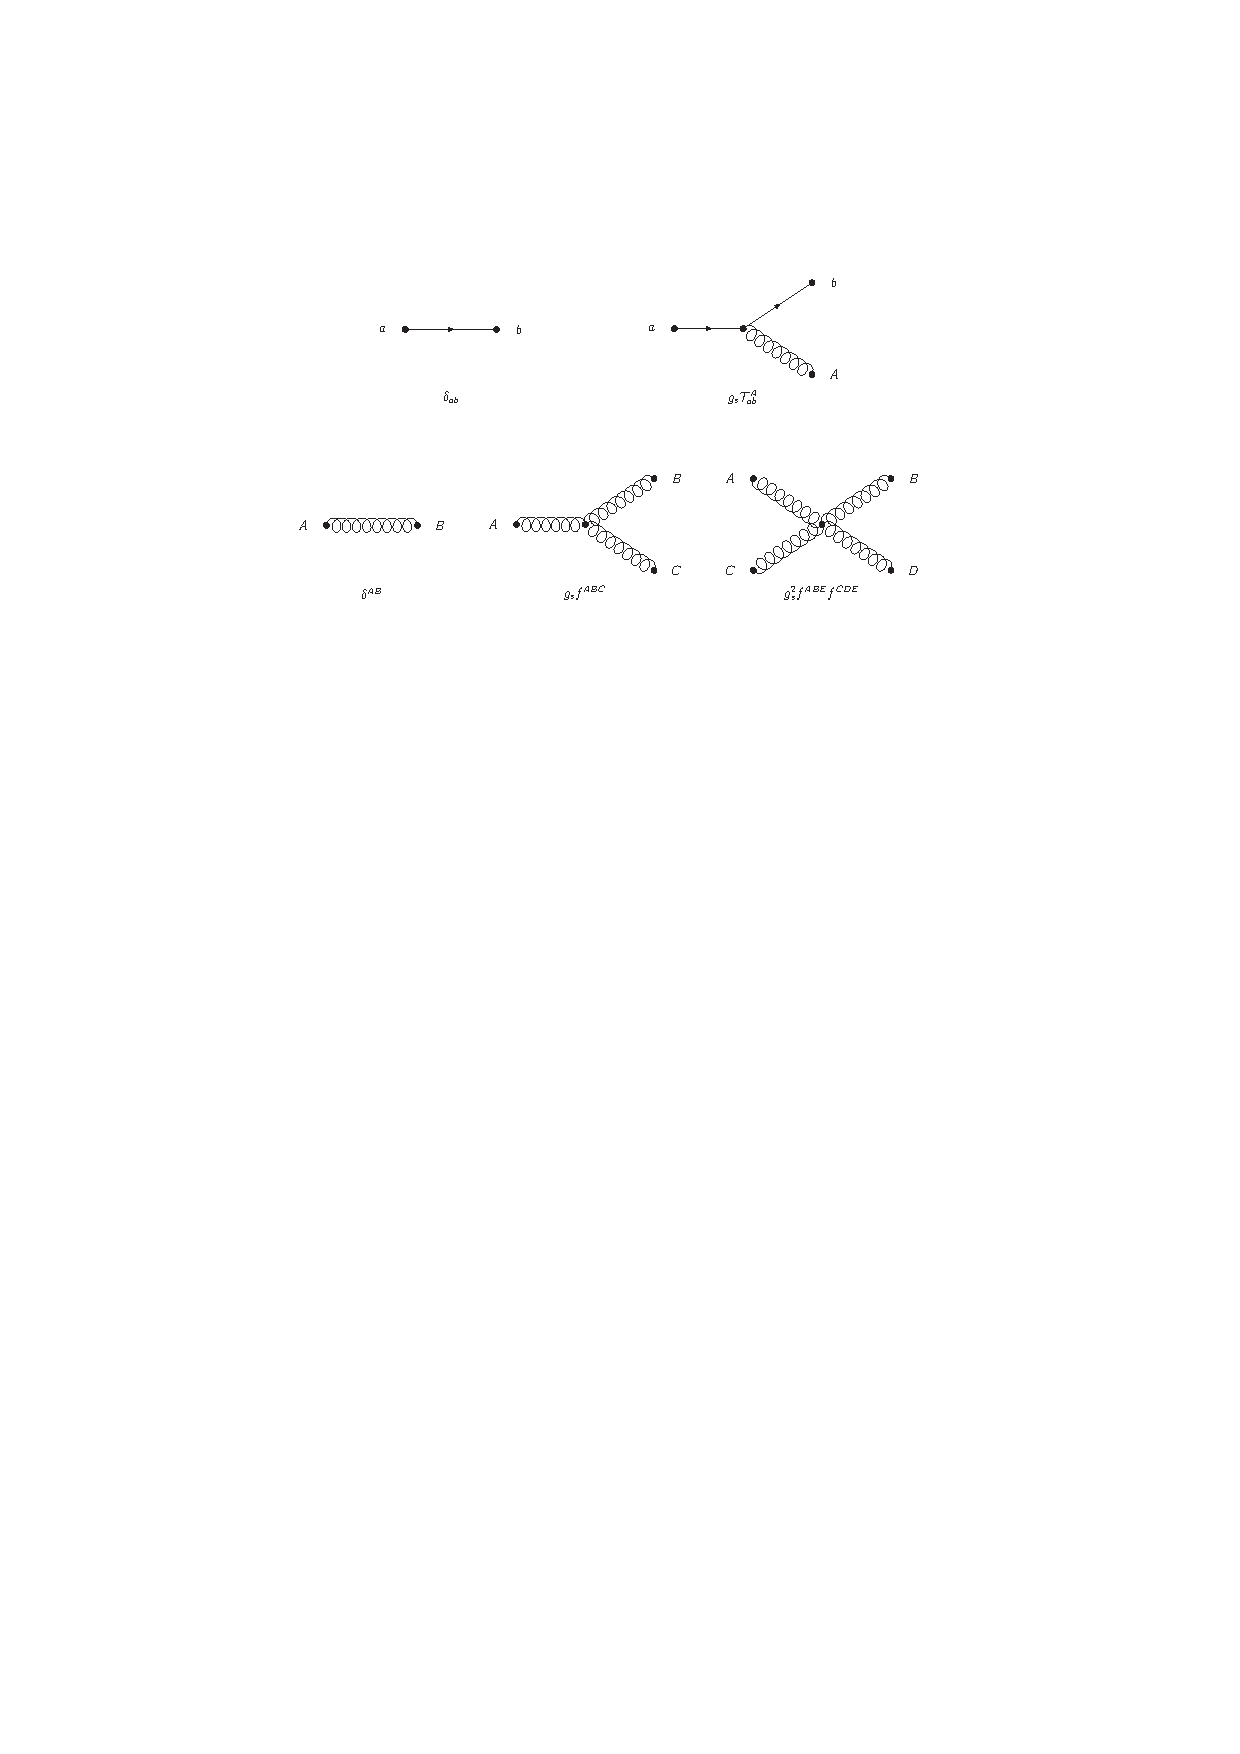
\includegraphics[width=0.95\textwidth]{/home/anter/Desktop/Thesis/Figures/edited_cropped_Feynmann.pdf}\\
\vspace*{4mm}
\caption[The fundamental Feynman rules of QCD.]{The fundamental Feynman rules of a free quark-field term (top left), quark-gluon interaction term (top right), free gluon-field term (bottom left), cubic gluon self-interaction term (bottom middle) and quartic gluon self-interaction term (bottom right). Taken from \cite{Rabbertz:2017ssq}.}
\label{fig:feyn}
\end{center}
\end{figure}

It is impossible to use perturbation theory on a gauge invariant Lagrangian without choosing a specific gauge in which to calculate. The usual gauge-fixing term is given by 
\begin{equation}
{\cal L}_{gauge}=-\frac{1}{2\xi} (\partial^{\mu}{\cal A}^{A}_{\mu})^{2}
\label{eq:gauge-fixing}
\end{equation}
where $\xi$ may be any finite constant. This choice fixes the class of covariant gauges with $\xi$ as the gauge parameter. As QCD is non-abelian, the gauge fixing term must be supplemented by a ghost Lagrangian as
\begin{equation}
{\cal L}_{ghost}=\partial_{\alpha}\eta^{A\dagger}(D^{\mu}_{AB}\eta^{B})
\label{eq:ghost}
\end{equation}
where $\eta^{A}$ is a complex scalar field which obeys Fermi-Dirac statistics. The ghost fields cancel unphysical degrees of freedom arising due to use of covariant gauges. This completes the QCD Lagrangian shown in Eq.~\ref{eq:lag}.

The strength of an interaction is given by a fundamental parameter called the coupling constant $\alpha$. In QED, the coupling constant $\alpha_e$ = $e^2/4\pi$ = 1/137 is constant. In contrast to this, in QCD, the coupling constant \alpsq = $g^2_s/4\pi$ is not constant and depends on the separation between the interacting particles. It increases with the increase in the distance or decrease in the energy scale Q. At large distances or low energies, the quarks can never be found as free particles but exit in color neutral bound states known as hadrons. Hadrons are of two types : baryons and mesons. According to the quark model \cite{Griffiths:111880} every (anti-)baryon is made up of three (anti-)quarks and every meson is made up of a quark-antiquark pair. When the colored partons within a hadron are pulled farther and farther apart, there is an increase in the strength of force between them. This results in creation of new quark-antiquark pair making difficult to liberate a free quark or gluon. This property of QCD is known as confinement according to which at low energy, the partons are forever bound into hadrons such as protons ($uud$), neutrons ($udd$). Although the gluons are massless but the confinement leads to the finite range of the strong interactions. On the other hand, at small distances, the strength of coupling decreases. The quarks and gluons interact very weakly and are treated as free particles. This property is known as asymptotic freedom. This indicates that perturbative theory is only applicable at high energies or small distances.

\subsection{Perturbative Quantum Chromodynamics}
At high energies, the property of asymptotic freedom allows a perturbative treatment in QCD calculations. In perturbative Quantum Chromodynamics (pQCD), any physical observable $X$ such as cross-section of a scattering process, can be expanded as a perturbative series in terms of coupling constant \alps as : 
\begin{equation}
X = \sum\limits_{i=0}^{N} \alpha^n_s {\rm c}_i = {\rm c}_0~\plus \alpha^1_s {\rm c}_1~\plus \alpha^2_s {\rm c}_2~\plus ...
\end{equation} 
where ${\rm c}_i$ are the perturbative coefficients. In a process, the pQCD calculation of X is determined by summing over the amplitudes of all Feynman diagrams contributing to that process. For a given Feynman diagram, the power of \alps is determined by the number of vertices associated with quark-gluon or gluon-gluon interactions. A leading order (LO) prediction sums over only the lowest-order contribution whereas next-to-leading order (NLO) includes terms with the additional powers of \alps. The next-to-next-to-leading order (NNLO) includes emission of another gluon or a virtual gluon loop. The different order of the QCD processes are shown in Fig.~\ref{fig:orders}.
\begin{figure}[!h]
\begin{center}
\hspace*{-1mm}
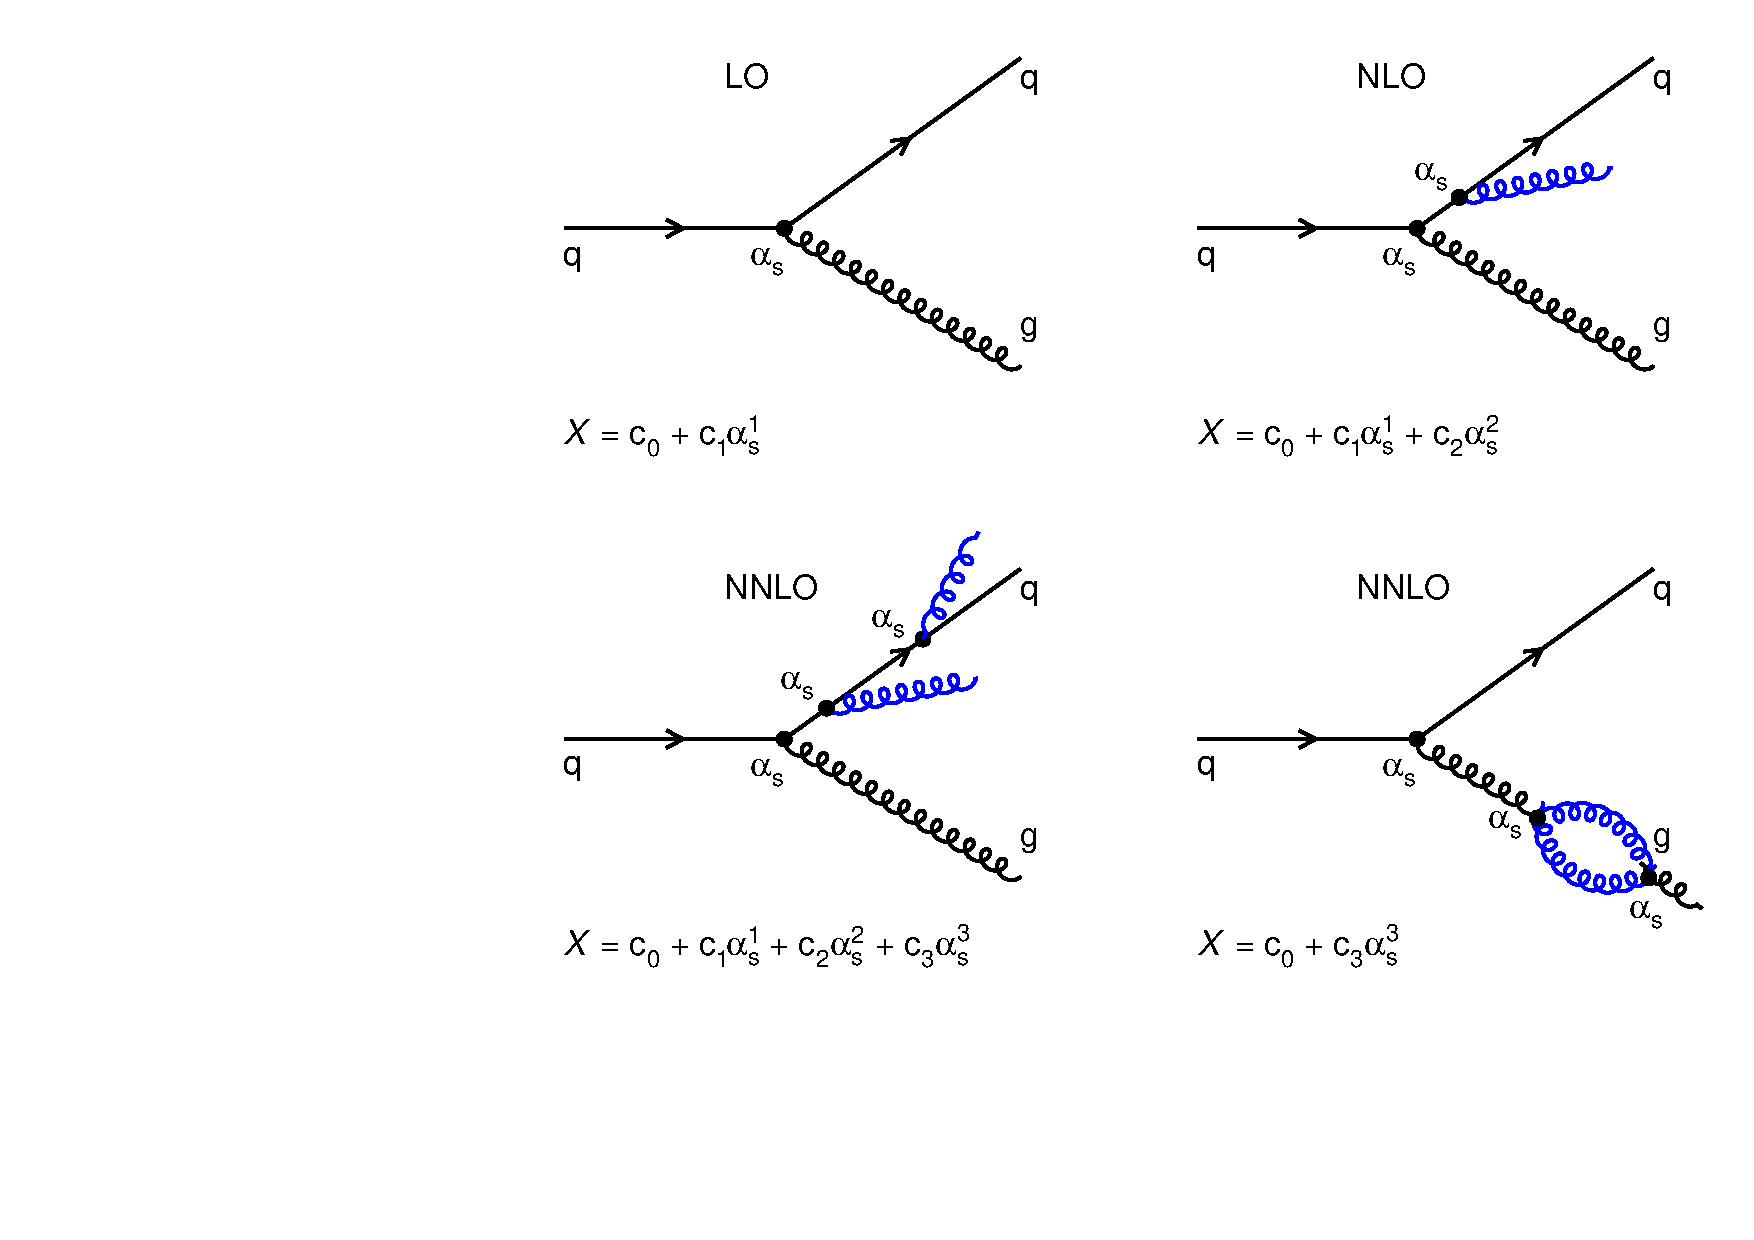
\includegraphics[width=0.95\textwidth]{/home/anter/Desktop/Thesis/Figures/Orders.pdf}\\
\vspace*{4mm}
\caption[The Feynman diagrams of leading-order (LO), next-to-leading order (NLO) and next-to-next-to-leading order (NNLO) processes in quantum chromodynamics.]{The Feynman diagrams\footnotemark of leading-order (LO), next-to-leading order (NLO) and next-to-next-to-leading order (NNLO) processes in quantum chromodynamics along with the perturbative expansion of any observable $X$ in powers of the strong coupling constant \alps. At each successive step in perturbation series, the emission of an additional gluon take place.}
\label{fig:orders}
\end{center}
\end{figure}
The calculations become complex with the loop diagrams where the momenta of the virtual particles in a loop are not fully constrained by four-momentum conservation and the associated integrals are divergent. Such ultraviolet (UV) divergences enter the calculations beyond LO either due to loop or vertex corrections. These are overcome by a procedure known as renormalization, described in next section. Apart from the UV divergences, the QCD also suffers from infrared and collinear divergences (IRC) due to the presence of massless gluons and neglected quark masses. These need to be handled in pQCD calculations. The observable to be studied must be IRC safe. 
\footnotetext{Drawn using ROOT}
\subsection{Renormalization and Running of the Strong Coupling}
The renormalization is a mathematical procedure which allows the finite calculation of momenta integrals of virtual loop by removing UV divergences. It introduces a regulator for the infinities, the renormalization scale \mur. At first, the divergences are regularized temporarily by introducing a cut-off to the loop momenta at \mur scale. Then the free parameters of the Lagrangian, i.e. the coupling constant are redefined or renormalized to absorb the UV divergences. Due to this, both \alpsq and observable $X$ become a function of \mur. The exact dependence of \alpsmusq on \mur is described by the renormalization group equation (RGE) which determines the running of \alpsmusq. According to RGE, the dependence of $X$ on \mur must cancel. Mathematically this can be expressed as : 
\begin{equation}
\mur^{2}\frac{d}{d\mur^{2}}X\Bigg(\frac{Q^{2}}{\mur^{2}},\alpha_{s}(\mur^{2})\Bigg)=
\Bigg(\mur^{2}\frac{\partial}{\partial\mur^{2}}~\plus \mur^{2}\frac{\partial\alpha_{s}(\mur^{2})}
{\partial\mur^{2}}\frac{\partial}{\partial\alpha_{s}(\mur^{2})}\Bigg)X=0
\label{eq:dmu}
\end{equation}
Using beta function $\beta(\alps)$ = $\mur^{2}\frac{\partial\alpha_{s}(\mur^{2})}{\partial\mur^{2}}$, Eq.~\ref{eq:dmu} can be re-written as 
\begin{equation}
\Bigg(\mur^{2}\frac{\partial}{\partial\mur^{2}}~\plus \beta(\alps)\frac{\partial}{\partial\alpha_{s}(\mur^{2})}\Bigg)X=0
\label{eq:dmu2}
\end{equation}
By setting the renormalization scale equal to the physical scale i.e. $\mu^{2}=Q^{2}$, $X\big(1,\alpha_{s}(Q)\big)$ is a solution to above equation. $Q$-dependence of the $X$ is only from the renormalization of the theory which is present in the classical theory. Hence measuring the $Q$-dependence of $X$ will directly probe the quantum structure of the theory. The $\beta$ function in QCD has a perturbative expansion as : 
\begin{equation}
\beta(\alps)=-\alpha_{s}^{2}\Big(b_0~\plus b_1\alps~\plus b_2\alpha_{s}^{2}~\plus {\cal O}(\alpha_{s}^{3})\Big) 
\label{eq:beta}
\end{equation}
where $b_n$ is the $n$\plus 1-loop $\beta$-function coefficients giving the dependence of the coupling on the energy scale $Q$. In the modified minimal subtraction ($\overline{\rm MS}$) scheme \cite{tHooft:1973mfk,Weinberg:1951ss}, the beta coefficient functions have following values :
\begin{equation}
b_0 = \frac{33-2n_f}{12\pi}, ~~~b_1 = \frac{153-19n_f}{24\pi^2}, ~~b_2 = \frac{77139 - 15099n_f~\plus 325n^2_f}{3456\pi^3}
\end{equation}
where $n_f$ is the number of quark flavours with masses $m_q$ \ls \mur. On integration of Eq.~\ref{eq:beta}, the energy dependence of \alps is yielded. Neglecting the higher orders, the first order solution of RGE is :
\begin{equation}
\alpha_{s}(\mur^2)=\frac{1}{b_0~{\rm ln}(\mur^2/\Lambda^2_{QCD})}
\label{eq:sol}
\end{equation}
where $\Lambda_{QCD}$ is the constant of integration. The perturbative coupling becomes large at the scale $\Lambda_{QCD}$ and the perturbative series diverge. With $b_0$ \gr 0, the coupling becomes weaker at higher scales $Q$, i.e. the effective color charge is small at small distances or large energies. This allows the quarks to behave as free particles within the hadron, leading to the property called asymptotic freedom. It is always convenient to express \alps at some fixed scale. Since some of the best measurements come from $Z^0$ decays, it is common practise to determine the strong coupling at the scale of the $Z$ boson mass \alpsmz. So, Eq.~\ref{eq:sol} can be expressed as :
\begin{equation}
\alps\bigg(\mur,\alpsmz\bigg) = \frac{\alpsmz}{1\plus\alpsmz b_0{\rm ln}(\mur^2/M^2_z)}
\end{equation}

Since \alps is the free parameter of QCD theory, it is always extracted from the experimental measurements and evolved to the scale of the $Z$ boson. According to Particle Data Group (PDG) \cite{Patrignani:2016xqp}, the current world average value of the strong coupling constant at the scale of mass of $Z$ boson is 
\begin{equation}
\alpsmz = 0.1181 \pm 0.0011
\end{equation}
This value is derived using data from deep inelastic scattering process, electron-positron annihilation processes, hadronic $\tau$ lepton decays, lattice QCD calculations and electroweak precision fits. The different experimental determinations of the strong coupling constant evolved at the scale $Q$ are shown as a function of $Q$ in Fig.~\ref{fig:alpha_pdg} which describe the running of the \alps up to the 1 TeV scale.
\vspace*{2mm}
\begin{figure}[!h]
\begin{center}
\hspace*{-7mm}
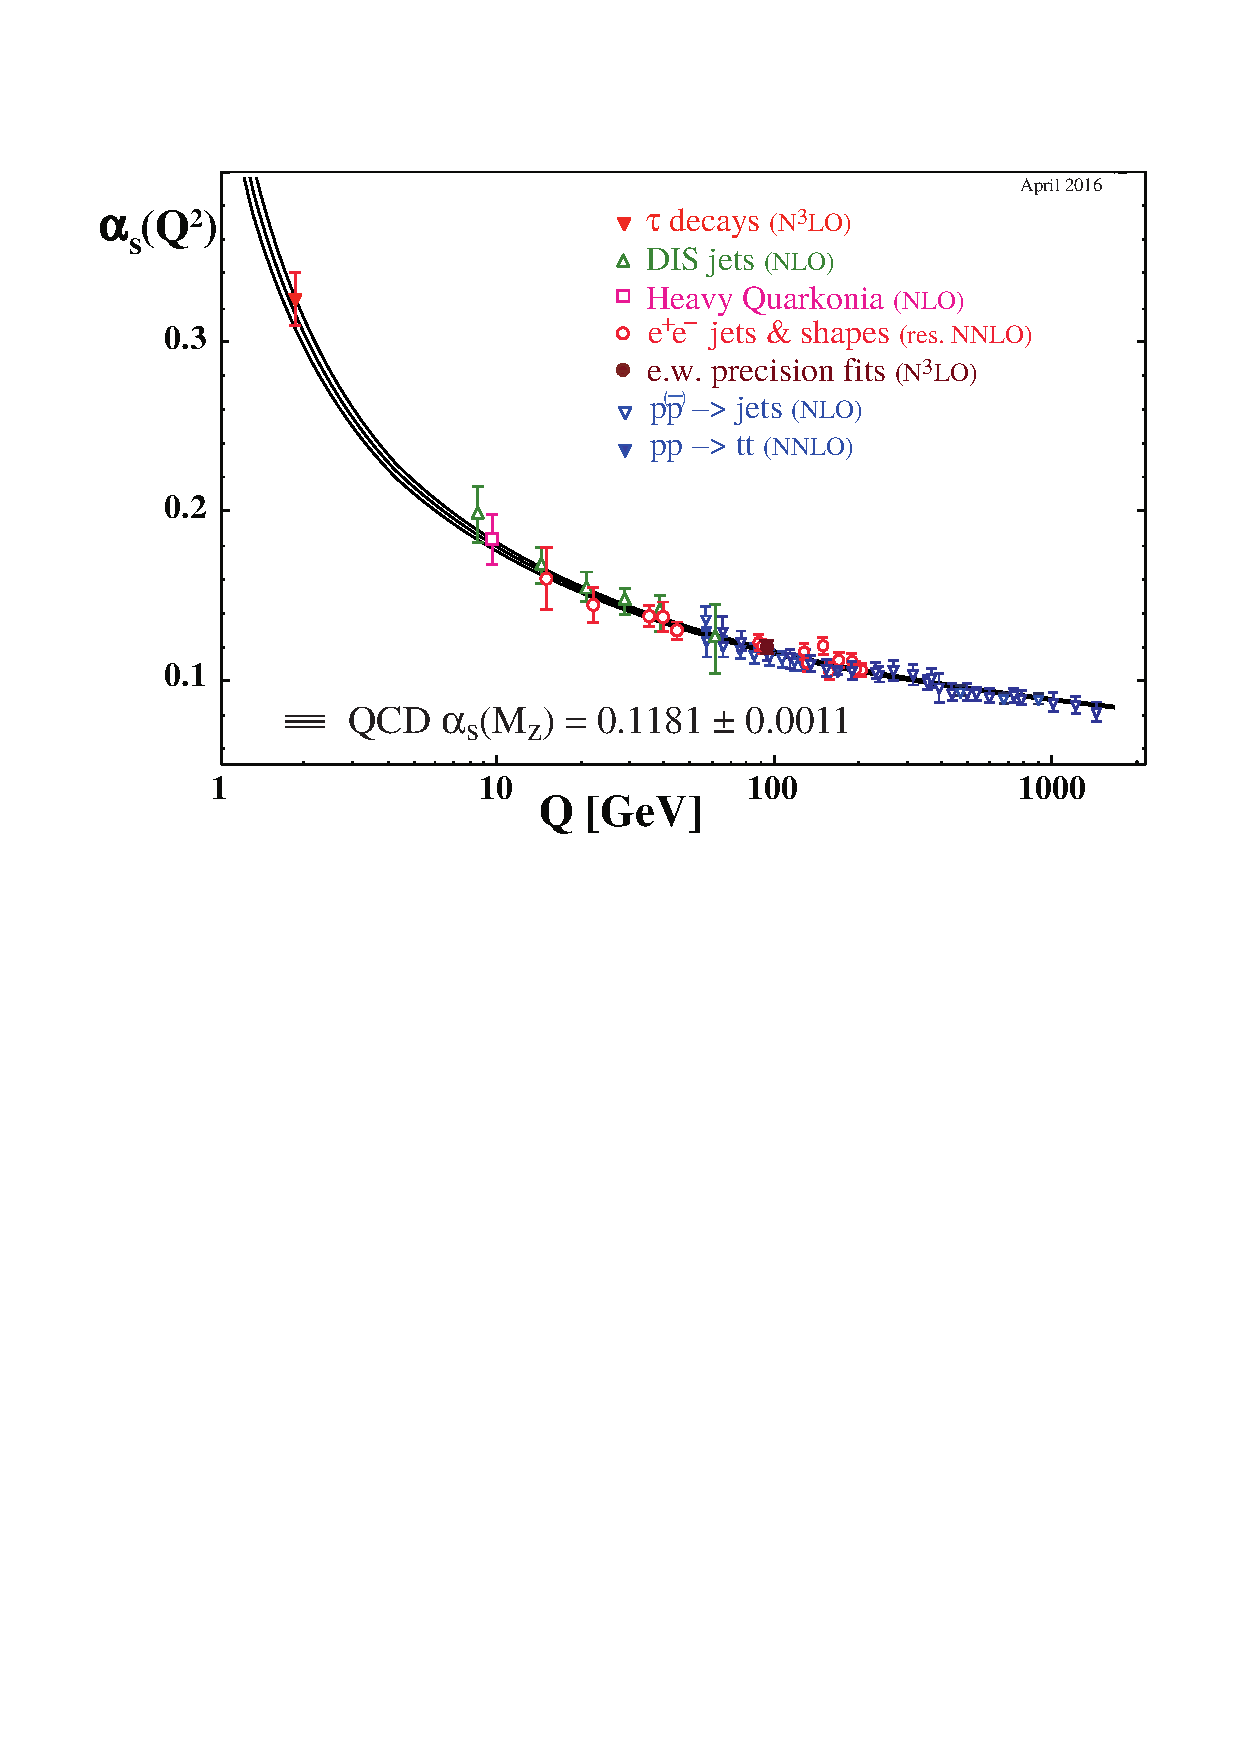
\includegraphics[width=0.95\textwidth]{/home/anter/Desktop/Thesis/Figures/cropped_Alpha.pdf}\\
\vspace*{4mm}
\caption[Running of the strong coupling constant.]{The different experimental measurements of the strong coupling constant \alps evolved at the energy scale $Q$ are shown as a function of $Q$. These describe the running of the \alps up to the 1 TeV scale. Taken from ~\cite{Patrignani:2016xqp}.}
\label{fig:alpha_pdg}
\end{center}
\end{figure}

\section{Hadronic Collisions}
At a large momentum transfer, the collision between two hadrons can be visualized as an interaction between their constituents - quarks and gluons. In this thesis, we are studying the proton-proton collisions taking place at the Large Hadron Collider (LHC). A proton is a complex composite particle consisting of three valence quarks ($uud$), gluons for the exchange of the strong force and the sea quarks. The sea quarks consist of quark-antiquark pairs coming into and out of existence rapidly and continuously due to gluon colour field splitting. In any collision, one of the most important quantities to evaluate is the cross-section ($\sigma$) of a certain process which gives the probability that the two hadrons interact and give rise to that specific process. In a hadronic collision, the perturbation theory is only valid at the parton-level but due to property of confinement at low energies, free partons cannot exist in nature. Only hadrons with a complex internal structure are available for the high energy collisions. Here, a factorization theorem of QCD \cite{Collins:1989gx} comes into play which allows the calculation of $\sigma$ by separating into two parts : a short-distance partonic cross-section calculable with pQCD, and a non-perturbative long-distance part described by parton distribution functions $f_i(x,\muf)$ (PDFs). The PDFs describe the partonic content of the colliding hadrons and give the probability to find a parton $i$ with momentum fraction $x$ within a hadron. \muf is a factorization scale which corresponds to the resolution with which the hadron is being probed. The particles which are emitted with transverse momenta \pt \gr \muf are considered in the calculation of hard scattering perturbative coefficients. The particles emitted with \pt \ls \muf are accounted for within the PDFs. Applying the factorization theorem in a proton-proton collision, the cross-section of a hard scattering process can be written as :
\begin{equation}
\begin{gathered}
\sigma_{P_1P_2 \rightarrow X} = \sum\limits_{i,j}^{}\int_{}^{} dx_1dx_2f_{i,P_1}(x_1,\muf)f_{j,P_2}(x_2,\muf)\\\times~\hat\sigma_{ij\rightarrow X} \Bigg(x_1p_1,x_2p_2,\alpha(\mur^2),\frac{Q^2}{\muf^2}\Bigg)
\end{gathered}
\end{equation}
where $f_i$ and $f_{j}$ are the proton PDFs which depend on momentum fractions $x_1$ and $x_2$ of parent protons $P_1$ and $P_2$ respectively as well as on the factorization scale \muf. The sum extends over all contributing initial-state parton flavours $i,~j$. The cross-section for the production of final state $X$ at parton level ($\hat\sigma_{ij}$) depends on the final state phase, the factorization scale \muf and the renormalization scale \mur. Figure.~\ref{fig:fac} illustrates the factorization into the PDFs and the hard scattering cross-section in a proton-proton collision.
\begin{figure}[!h]
\begin{center}
\hspace*{-7mm}
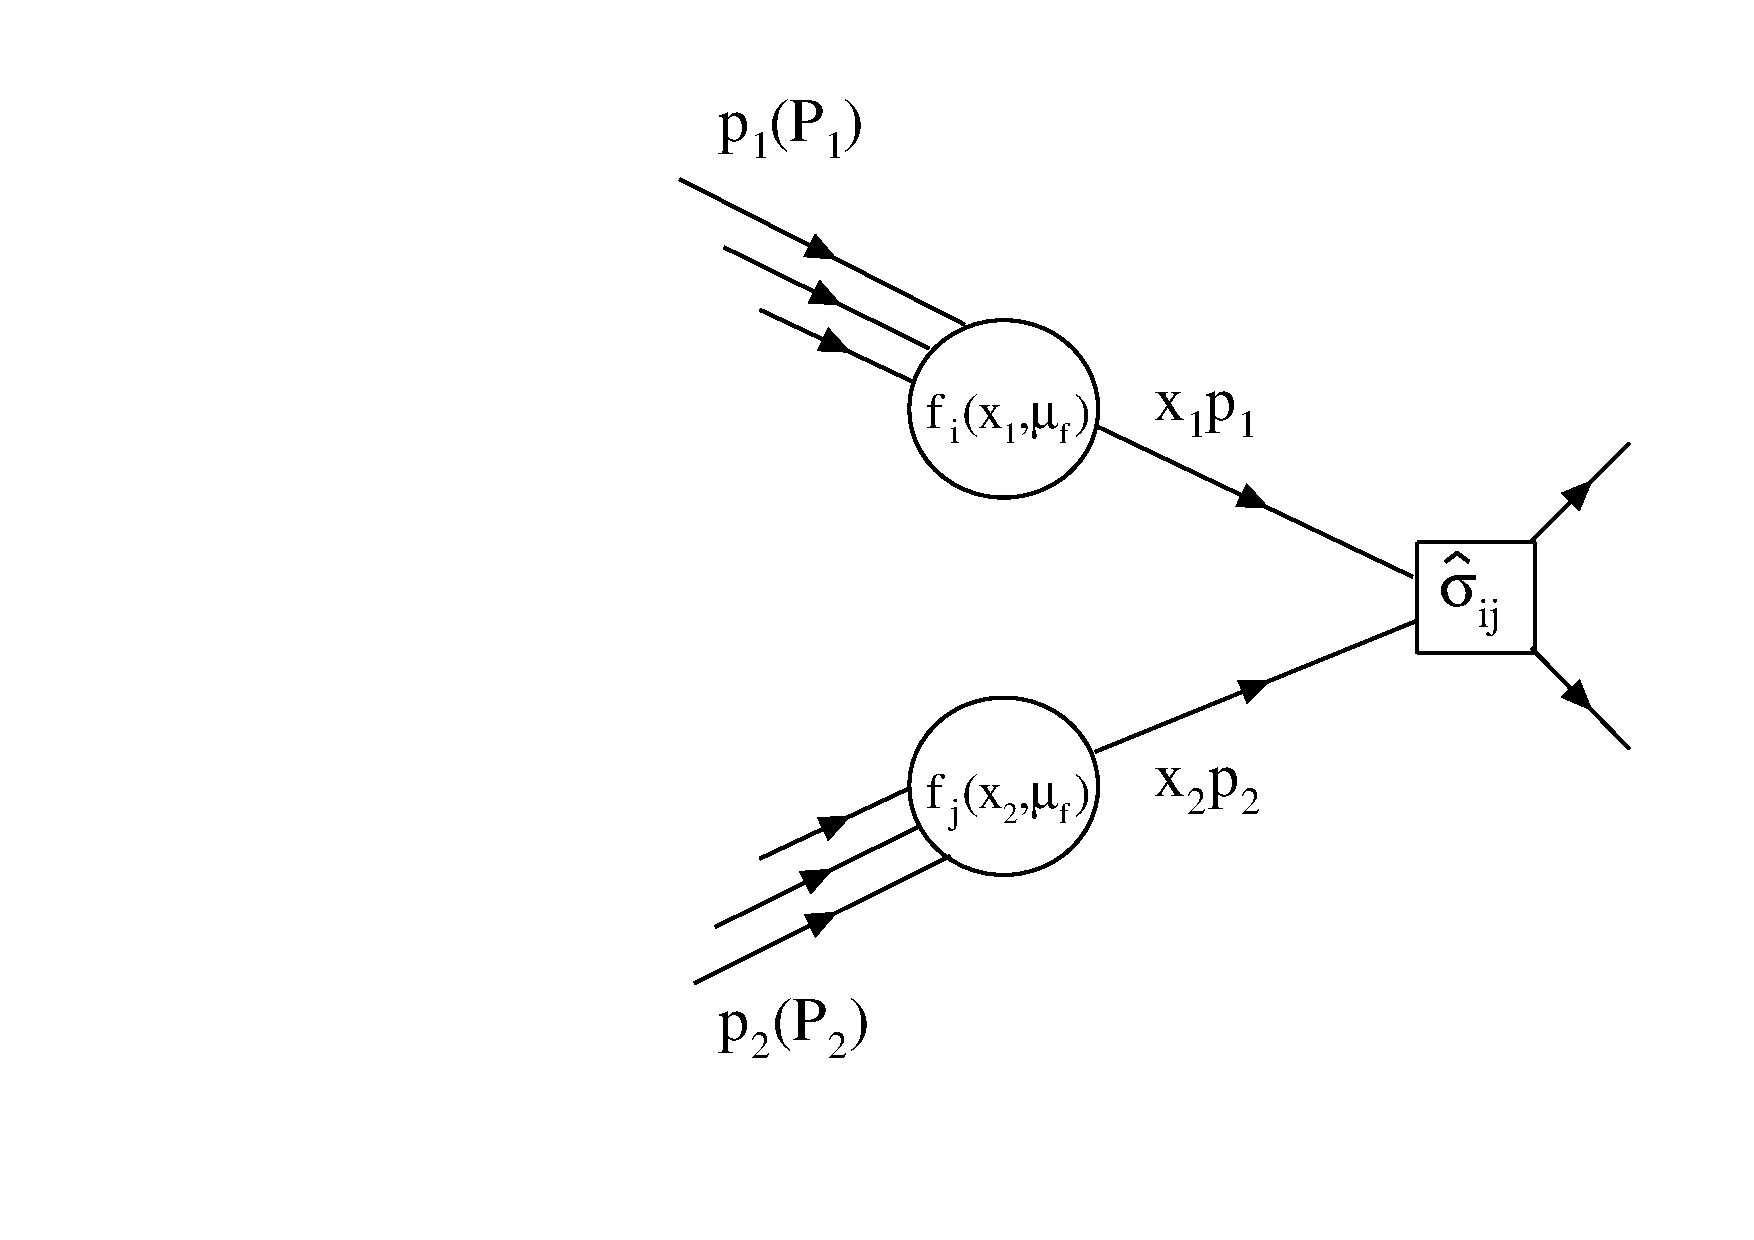
\includegraphics[width=0.65\textwidth]{/home/anter/Desktop/Thesis/Figures/Factorization.pdf}\\
\vspace*{4mm}
\caption[Schematic illustration of factorization theorem in a collision of two protons.]{Schematic illustration\footnotemark of the factorization theorem in a collision of two protons P1 and P2 having momenta p1 and p2, respectively. In a hard-scattering process at a scale $Q^2$, the two partons $x_1$ and $x_2$ participate with momenta $x_1p_1$ and $x_2p_2$. The total cross-section is factorized into the hard scattering cross-section $\hat\sigma_{ij}$ calculable using perturbative Quantum Chromodynamics and the PDFs $f_i(x_1,\muf)$ and $f_j(x_2,\muf)$ with factorization scale \muf.}
\label{fig:fac}
\end{center}
\end{figure}
\footnotetext{Drawn using ROOT}
The PDFs of the proton are a necessary input to almost all theory predictions of a proton-proton collision. The QCD does not predict the parton content of the proton. So the shapes of PDFs are determined in fits to experimental measurements of different experiments. The dependence of PDFs on \muf is given by the Dokshitzer-Gribov-Lipatov-Altarelli-Parisi (DGLAP) \cite{Gribov:1972ri,Dokshitzer:1977sg,Altarelli:1977zs} equations which use \alps and the RGE as inputs. The knowledge of proton PDFs mainly comes from the Deep Inelastic Scattering (DIS) HERA, fixed target and Tevatron data. The LHC data has a potential to improve constraints of the PDFs further as done in one of the recent CMS measurements \cite{Sirunyan:2017skj}. There are several groups which determine the PDFs using the different minimization methods, phenomenological approaches and the methods to estimate the uncertainties. The global PDFs are the CTEQ \cite{Dulat:2015mca}, MMHT \cite{Harland-Lang:2014zoa}, NNPDF \cite{Ball:2014uwa}, ABM \cite{Alekhin:2012ig} and HERAPDF \cite{Abramowicz:2015mha} at LO, NLO and NNLO.
%Source : \url{https://arxiv.org/pdf/1003.0521.pdf}}

\subsection{Parton Shower and Hadronization}
The partons involved in a hard scattering process get accelerated due to large momentum transfers. These accelerated partons emit QCD radiation in the form of gluons with successively lower energy. Unlike the uncharged photons in QED, the gluons themselves carry color charge and hence also emit further gluons. The emitted gluons in turn splits into $q\bar{q}$ pairs. This successive emission of partons lead to a parton shower. In a parton shower, the main contribution is by the collinear parton splitting and the soft gluon emissions. The parton shower mimics the effect of higher-order corrections to the hard process. These cannot be calculated exactly and are taken into account using the parton shower approximation. The two incoming partons which are constituents of two colliding hadrons and taking part in hard scattering process can also develop parton showers, commonly known as Initial-State Radiation (ISR). The initial partons produce showers till they collide to initiate the hard scattering process. The final outgoing partons produced from a hard scattering process can also undergo parton showering giving rise to Final-State Radiation (FSR). A parton shower terminates when the scale $Q$ is below the hadronization scale $\sim$ 1 GeV for QCD.

At the end of the shower, there is a decrease in the energy of partons due to successive emission of gluons. Due to this the coupling constant of QCD \alps evolves and become large. This leads to the confinement of colored quarks and gluons into the color-neutral composite particles called hadrons and this process is known as hadronization. The hadronization takes place at low momentum transfer and hence non-perturbative in nature. Although no exact theory for hadronization is known, the different phenomenological models have been developed to simulate the hadronization process. The two main models implemented in Monte Carlo event generators to simulate the hadronization process are : \\\newline
{\bf Lund String Model -} In the Lund string model of hadronization \cite{Andersson:1998tv}, the highly energetic gluons are treated as field lines. Due to the gluon self-interaction, the gluons are attracted to each other forming a narrow tube or string of strong color field between a $q\bar{q}$ pair. This model is based on an observation that at distances greater than about a femtometer (fm), the potential energy $V(r)$ of colored quarks grows linearly with the increase in distance between them ($r$) as :
\begin{equation}
V(r) = \kappa r
\end{equation}
where $\kappa \sim {\rm GeV/fm^2}$ is the tension of the string connecting the quarks. When the $q$ and $\bar{q}$ are pulled apart from each other move apart, the gluonic string stretches. Due to this, the potential energy of the string grows at the expense of the kinetic energy of the quarks. As the potential energy becomes of the order of hadron masses, the string breaks at some point along its length, creating a new $q\bar{q}$ pair. The newly formed two string segments again stretch and break producing further $q\bar{q}$ pairs. This process of stretching and breaking continues until all the potential energy gets converted to $q\bar{q}$ pairs. This whole process is illustrated in Fig~\ref{fig:string}. The $q\bar{q}$ pairs then undergo hadronization due to confinement property. \PYTHIA~Monte Carlo generator uses the Lund string model. \\ \newline
{\bf Cluster Model -} The cluster model of hadronization \cite{Marchesini:1987cf,Webber:1983if} is based on preconfinement property of QCD \cite{Amati:1979fg}. According to this property, at evolution scales $Q_0$ much less than the hard process scale $Q$, the partons produced in a shower are clustered in colourless groups with an invariant mass distribution, depending on nature of hard process and $Q_0$, not on $Q$. This model contains two steps : firstly all gluons split into $q\bar{q}$ pairs at the end of the parton shower and in the second step, a new set of low-mass color-singlet clusters are obtained which decay into either secondary clusters or directly into hadrons. The generator \HERWIG~is based on the cluster fragmentation model. However, this model has problems in dealing with the decay of very massive clusters. 

\begin{figure}[!h]
\begin{center}
\hspace*{-4mm}
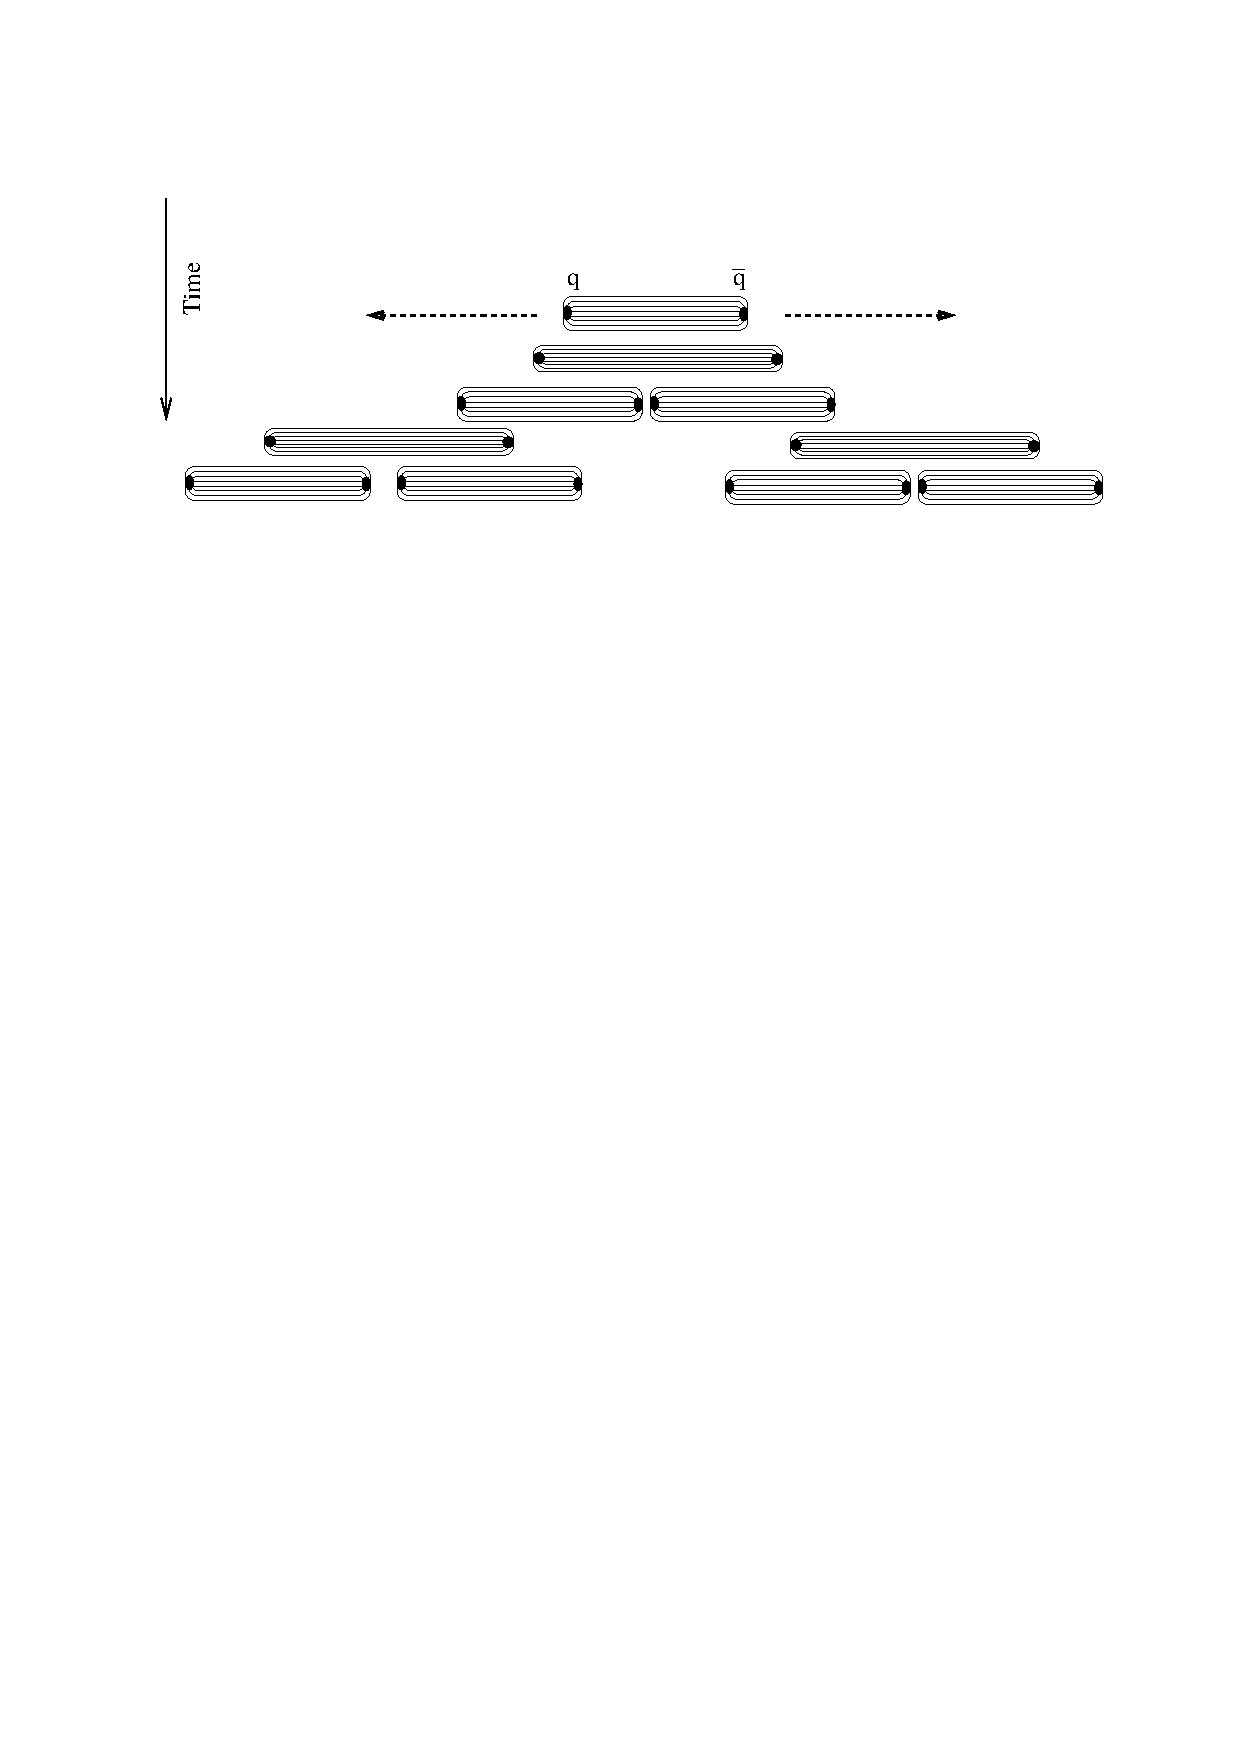
\includegraphics[width=0.95\textwidth]{/home/anter/Desktop/Thesis/Figures/cropped_String.pdf}\\
\vspace*{4mm}
\caption[Illustration of the hadronization process in Lund string model.]{Illustration of the hadronization process in Lund string model\footnotemark. When the quark $q$ and anti-quark $\bar{q}$ are pulled apart from each other, the potential energy of the gluonic string connecting the quarks increases. As it becomes of the order of hadron masses, the string breaks and a new $q\bar{q}$ pair is created. The breaking of string and creation of $q\bar{q}$ continues till all the potential energy gets converted to $q\bar{q}$ pairs which then get hadronized.}
\label{fig:string}
\end{center}
\end{figure}
\footnotetext{Source : \url{http://inspirehep.net/record/806744}}
\subsection{Underlying Event}
Due to the composite nature of the protons, their collisions are not clean events. The event structure is significantly more complex than that of the lepton collisions. The final states of the collisions involves the multiparticle calculations. In a high energy proton-proton collisions, the underlying event (UE) includes the effects which are not coming from the primary hard scattering process. The UE include the contributions from relatively small momentum transfer processes : initial and final-state radiations (ISR, FSR), leftover partons in the collisions called beam remnants and multiple parton interactions (MPI). Due to composite nature of proton, the remaining two partons which do not participate in a hard collision may also interact giving rise to multiple parton interactions. The UE induces an additional energy in an event which is not related to the main hard interaction. This acts an unavoidable background which needs to be removed. Hence, it is very crucial to study and understand the UE. The UE activity increases with $Q$ and the center-of-mass energy \cme. Figure~\ref{fig:MPI} shows the complex variety of processes taking place in a single proton-proton collision.

\begin{figure}[!h]
\begin{center}
\hspace*{-7mm}
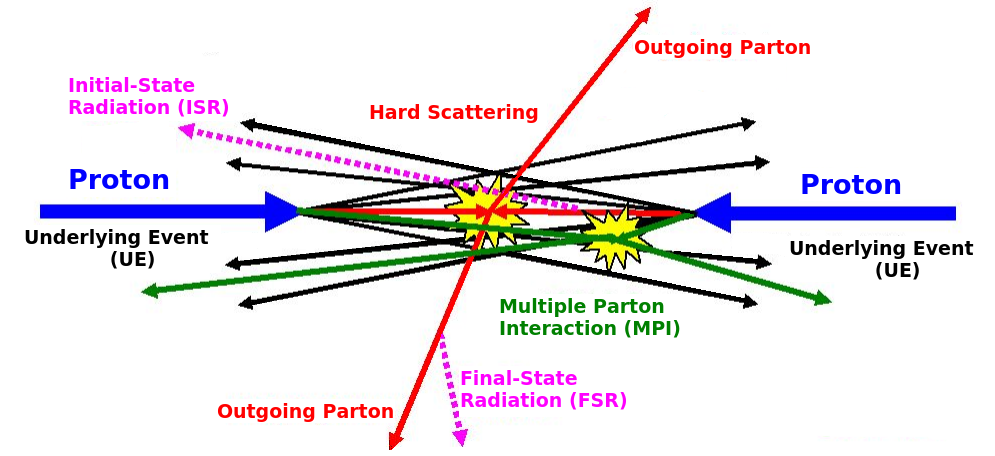
\includegraphics[width=0.95\textwidth]{/home/anter/Desktop/Thesis/Figures/MPI.png}\\
\vspace*{4mm}
\caption[Proton-proton collision.]{A proton-proton collision\footnotemark~involving the main hard scattering process along with the low momentum transfer underlying event (UE) contributions coming from initial- and final-state radiations (ISR and FSR) complemented with multiple parton interactions (MPI) and collisions from leftover partons called beam remnants.}
\label{fig:MPI}
\end{center}
\end{figure}
\footnotetext{Source : \href{https://www-cdf.fnal.gov/physics/new/qcd/ue_escan/}{The Energy Dependence of Min-Bias and the Underlying Event at CDF}}
The bunch of hadrons, produced from hadronization of quarks and gluons, gets collimated in the form of ``jets'' with the direction towards the direction of the initial parton that originated them. The jets are the final structures observed experimentally in the detectors. These act as a bridge between the elementary quarks and gluons of QCD and the final hadrons produced in high energy collisions. Therefore, at large momentum transfer of the interacting partons, the jets and their observables are the best tools to test the predictions of perturbative QCD. Also, the jet production is sensitive to the strong coupling constant \alpsns. The precise knowledge of the jet production cross-section can help to extract the value of \alps and also to reduce the uncertainties of the PDFs of proton. In LHC, the simplest jet production process is 2 $\rightarrow$ 2 scattering process at leading-order giving dijet events. But the partons originating from ISR, FSR or MPI can also hadronize to produce jets greater than 2 in a single proton-proton collision. This results in the production of multijet events. The investigation of inclusive multijet event cross-sections permits more elaborate tests of QCD. Also, a precise study of jet variables helps to understand the signal and background modelling for the new physics search in hadronic final states. In this thesis, the inclusive multijet event cross-sections as well as the ratio of cross-sections are exploited to extract the value of strong coupling constant \alps. In the next section, we focus on the definition of a jet.

\section{Jets}
\label{sec:jets}
Jets \cite{Sterman:1977wj} are the conical structures which group the hadrons into a single physics entity. Figure~\ref{fig:jet_r} shows the the outgoing partons of the hard scattering process in a proton-proton collision, undergoing fragmentation and hadronization processes and forming a conical jet with radius R. The jet structure was observed for the first time hadron production of $e^\plusn e^-$ annihilation process at SLAC in 1975 \cite{Hanson:1975fe}. The partons can not be measured directly by the experiments because they can not exist freely in nature. The information about the dynamics of the partons can be obtained indirectly from jets. The configurations of high-energy quarks and gluons at short distances are truly reflected in the energy and angular distributions of the jets. Hence the jets are important to study. To perform the clustering of particles, a certain set of rules are followed in the form of jet algorithms. 

\begin{figure}[!h]
\begin{center}
\hspace*{-7mm}
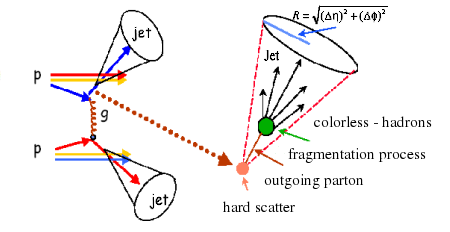
\includegraphics[width=0.75\textwidth]{/home/anter/Desktop/Thesis/Figures/jet2.png}\\
\vspace*{4mm}
\caption[Formation of a jet in a proton-proton collision.]{In a proton-proton collision, the outgoing partons of the hard scattering process undergo fragmentation and hadronization processes producing a shower of partons which get collimated into a conical jet with radius R.}
\label{fig:jet_r}
\end{center}
\end{figure}

\subsection{Jet Algorithms}
\label{sec:jet_algos}
Jet algorithms \cite{Salam:2009jx} provide a set of rules which determine how the particles can be clustered into a jet. In a jet algorithm, usually one or more parameters are involved that indicate how close two particles must be for them to belong to the same jet. These parameters can either measure closeness in coordinate space (cone algorithms) or in momentum space (sequential algorithms). The jet algorithms are applicable on parton, particle and calorimeter levels. A recombination scheme is always associated with a jet algorithm which calculates the momentum assigned to the combined particles. A jet algorithm along with its parameters and a recombination scheme forms a ``jet definition''. A jet definition \cite{Ellis:1989vm} must be simple to implement in an experimental analysis as well as in the theoretical calculation. It should be defined at any order of perturbation theory. It must yield finite cross-section at any order of perturbation theory that is relatively intensive to hadronization. In addition to these requirements, a jet algorithm must be infrared and collinear (IRC) safe. Infrared safety is the property by which the addition of a soft emission i.e. addition of a soft gluon should not change or modify the number of hard jets found in an event. In an infrared unsafe algorithm, a soft gluon emission in the middle of two cone jets can lead to overlap of the two initial cones, as shown in Fig.~\ref{fig:IRC} (top). This produces a single jet instead of initial two jets resulting in the change of number of jets. 
\begin{figure}[h!]
\begin{center} 
%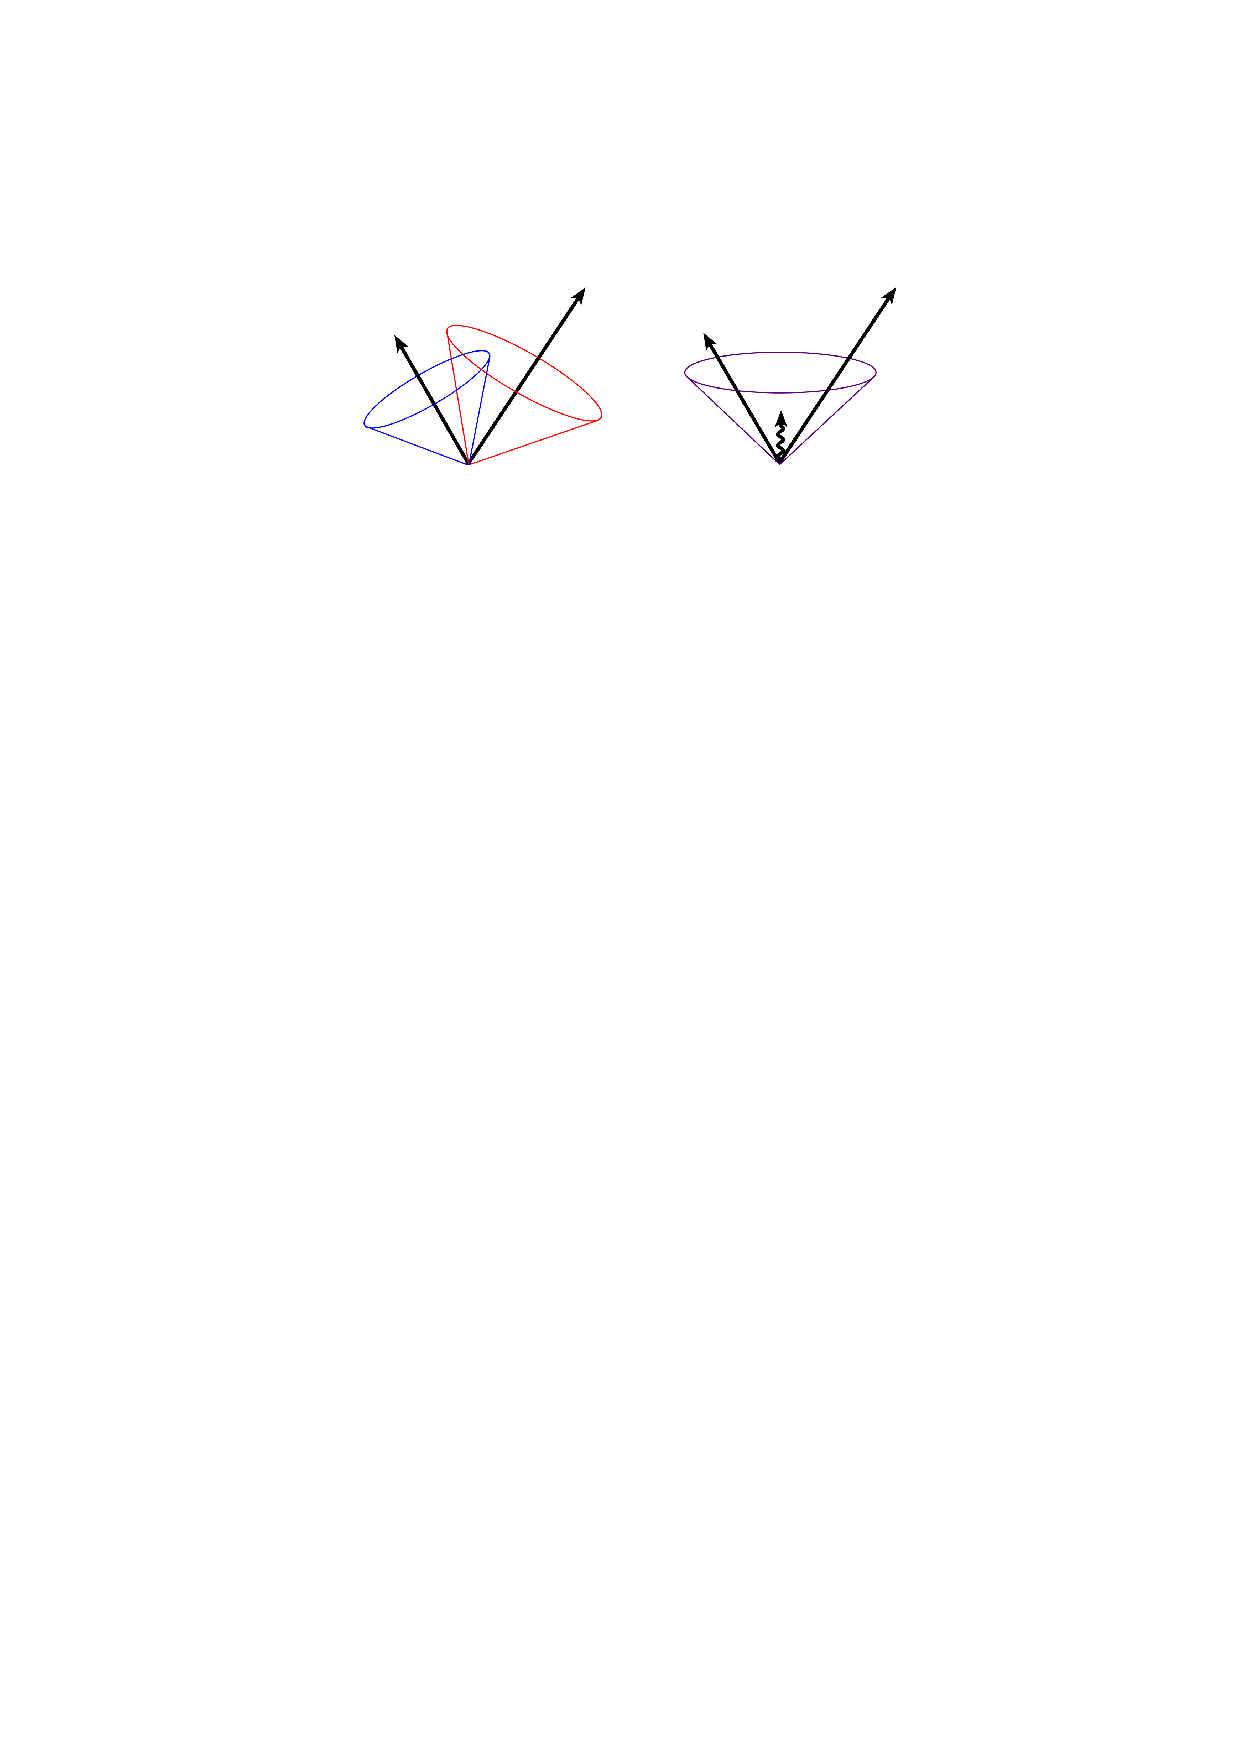
\includegraphics[scale = 1.3]{/home/anter/Desktop/Thesis/Figures/cropped_IR.pdf}\\
%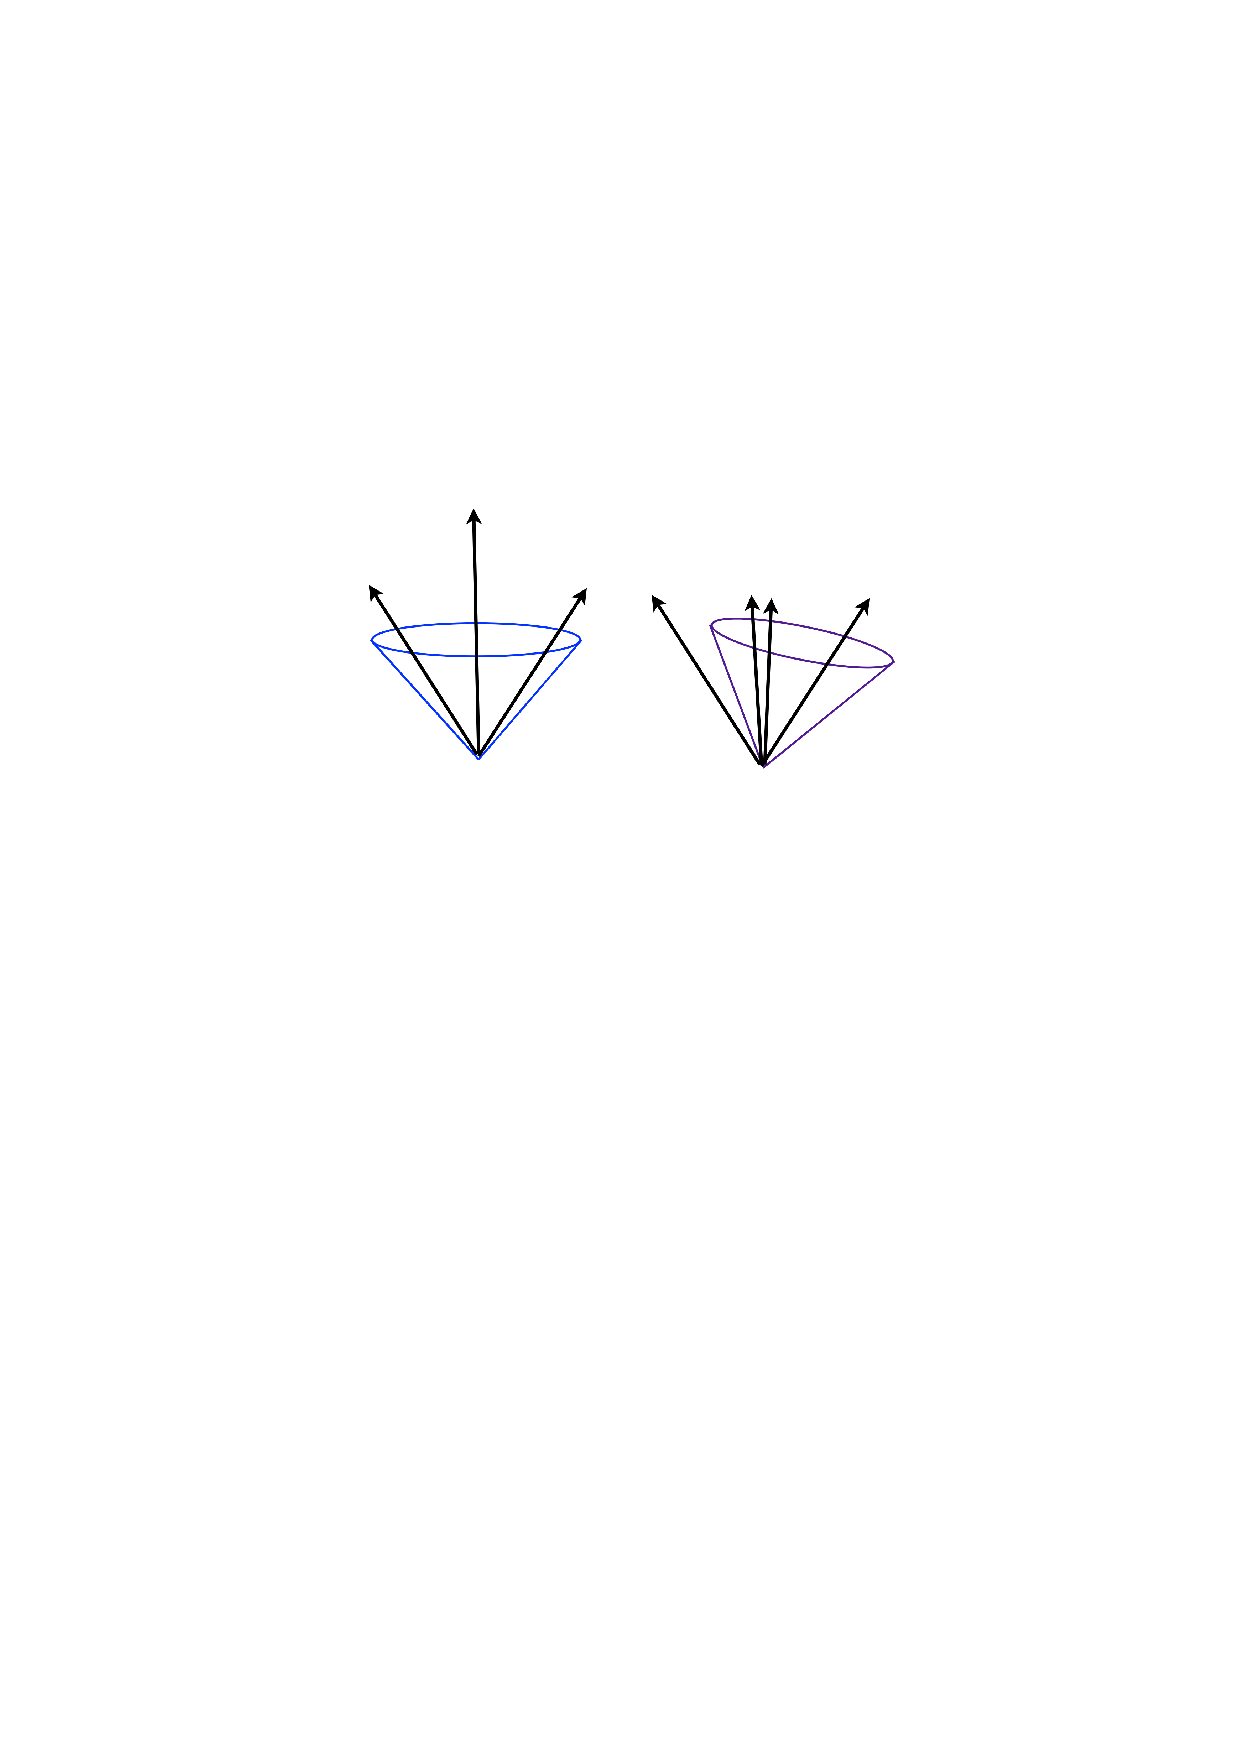
\includegraphics[scale = 1.1]{/home/anter/Desktop/Thesis/Figures/cropped_Collinear.pdf}
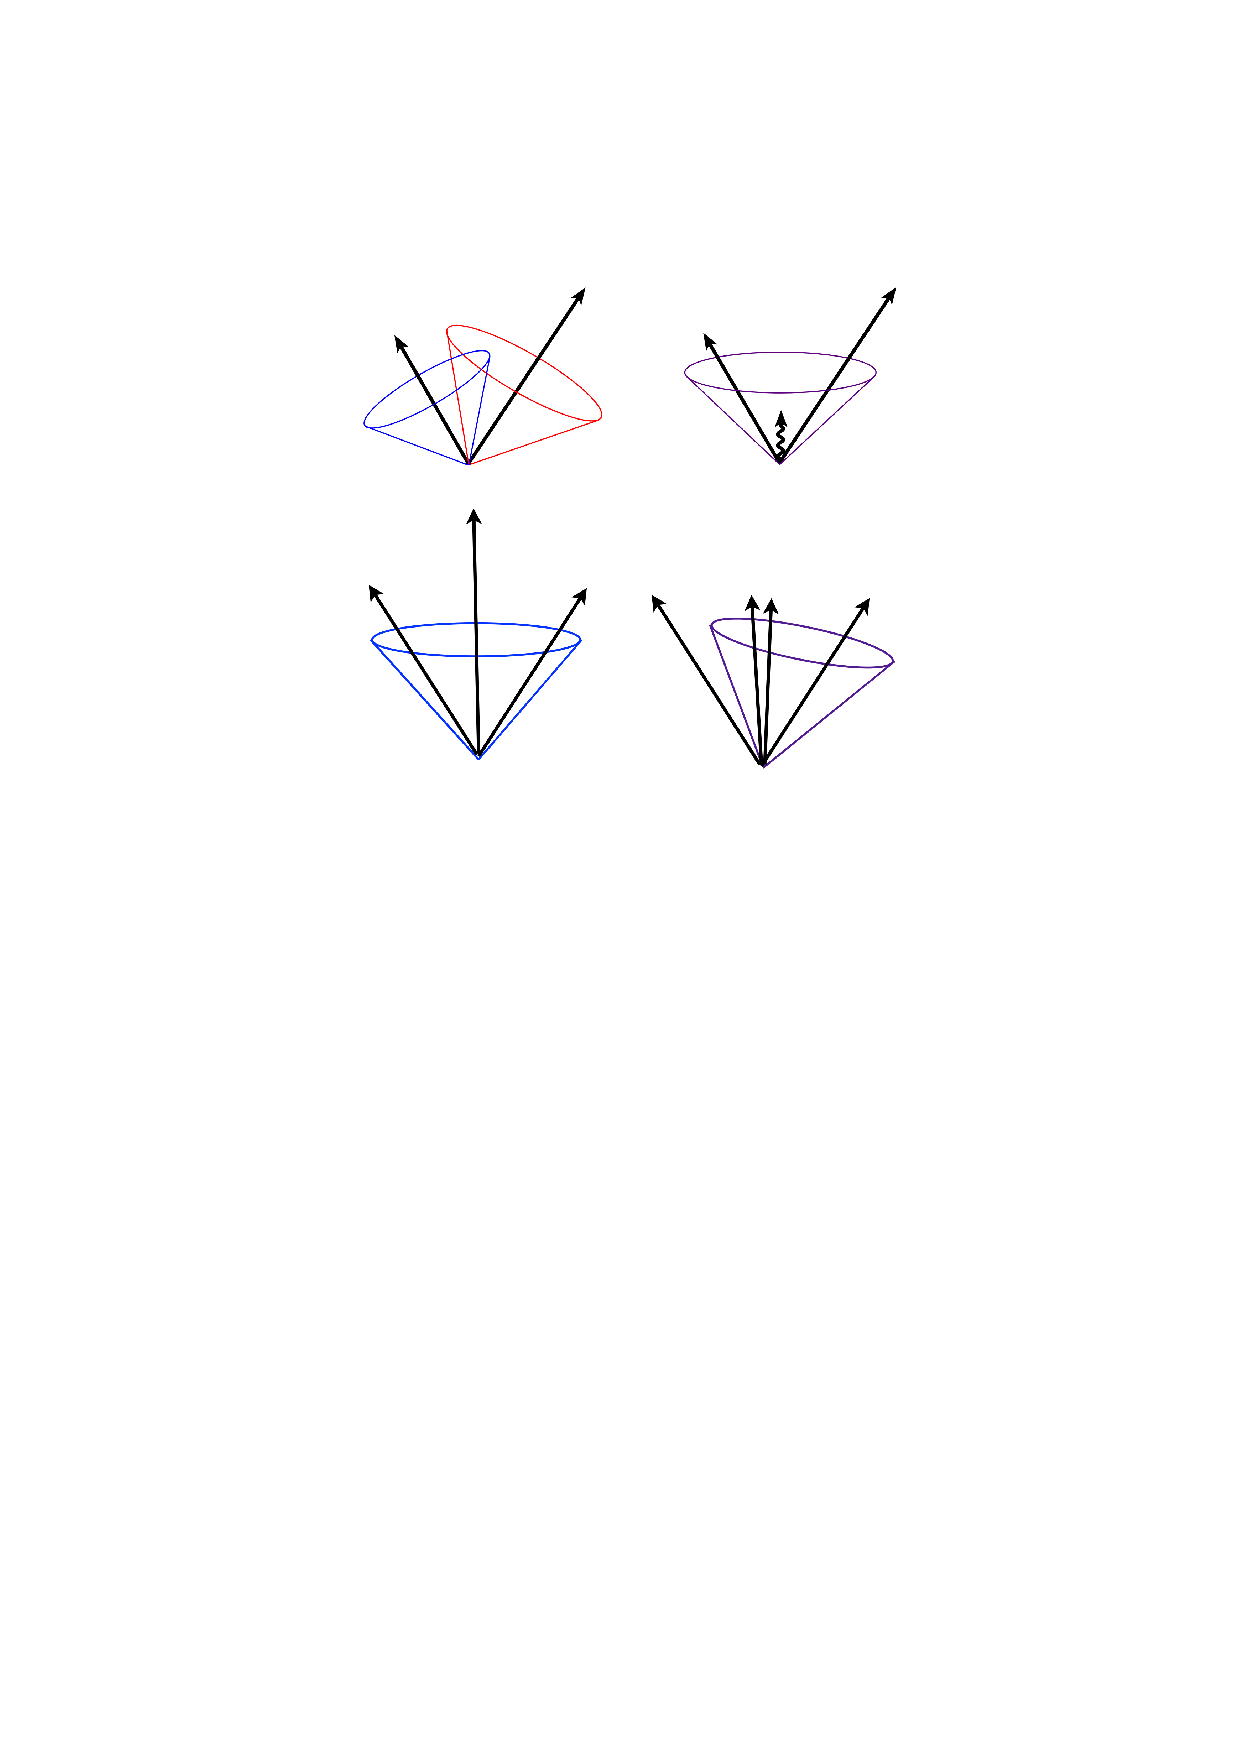
\includegraphics[scale = 0.9]{/home/anter/Desktop/Thesis/Figures/cropped_Algo.pdf}
\caption[Effects of emission of infrared radiations and collinear splitting in jet algorithms.]{Top : Infrared unsafe behavior of jet algorithm is illustrated where the presence of soft radiation between two jets may cause a merging of the jets that would not occur in the absence of the soft radiation. Bottom : Collinear unsafe behavior of jet algorithm is shown in which the number of jets change due to a collinear splitting\footnotemark.}
\label{fig:IRC}
\end{center}
\end{figure} \footnotetext{Source : \url{http://inspirehep.net/record/1251416}} Collinear safety is the property by virtue of which the collinear splitting i.e. replacement of one parton by two at the same place should not be modify the number of jets formed in a jet. This implies that the output of the jet algorithm should remain the same if the energy of a particle is distributed among two collinear particles. According to the collinear safety property, the two cases shown in Fig.~\ref{fig:IRC} (bottom) should always produce a single jet. If an algorithm produces zero or two jets after collinear splitting, then it is not collinear safe. 

The jet algorithms can be classified mainly into two types : \\ \newline
{\bf Cone algorithms -} In the iterative cone (IC) algorithm \cite{Blazey:2000qt}, the jet is defined as a cone with fixed radius $R$ in $\eta$-$\phi$ space drawn around the highest energy seed. The relative distance ($d$) of all the particles is iteratively calculated and compared with $R$. If the calculated $d$ \ls $R$, the considered particles are clustered together in a jet and the directions of the clustered particles give the direction of the jet. On the other side i.e. if $d$ \gr $R$, the considered particles initiate two different jets. The algorithm iterates until the cone is stable which means that the direction of sum of momentum of all the particles is same as that of the center of cone. But IC algorithm is not IRC safe. There is an another cone algorithm, Seedless Infrared-Safe cone (SIS-Cone) \cite{Weinzierl:2011jx}, which is an exact seedless i.e. does not rely on seed threshold and is IRC safe. This is a complex approach which tests the stability of all subsets of particles and has a complexity of ${\cal O}(N2^{N})$ for $N$ particles. But this algorithm is much slower and hence not preferred. \\ \newline
{\bf Sequential algorithms -} The sequential algorithms \cite{Ellis:1993tq} cluster the particles by defining a distance between pairs of particles and recombine the pair of closest particles successively. This is collinear and infrared safe algorithm. It is possible for the jet cones to overlap such that one particle is contained in more than one jet but the sequential algorithm never assigns a particle to more than one jet. The sequential algorithm is based on transverse momentum \pt of the particles and follows the below procedure : 
\begin{enumerate}
\item First the distance $d_{ij}$ between two particles $i$ and $j$ and distance $d_{iB}$ of the particle to the beam are calculated.
 \begin{equation}
\begin{gathered}
d_{ij} = {\rm min}\big(p^{2p}_{{\rm T}i},p^{2p}_{{\rm T}j}\big) \frac{\Delta R^2_{ij}}{R^2}, ~~~~d_{iB} = p^{2p}_{{\rm T}i} \\ {\rm where} ~~~\Delta R^2_{ij} = (\eta_i -\eta_j)^{2} ~\plus (\phi_i -\phi_j)^{2}
\end{gathered}
\end{equation}

\item If $d_{ij}$ \ls $d_{iB}$, then the particles $i$ and $j$ are merged into a new single particle $k$, summing four-momenta of two initial particles by recombination scheme and step 1 is repeated. 
\item If $d_{iB}$ \ls $d_{ij}$, particle $i$ is declared as a final-state jet and the particle gets removed from the list. 
\end{enumerate}
This procedure continues until all particles get clustered into jets. The value of the parameter $p$ defines the three different sequential algorithms having distinct properties. For $p$ = 1, we have \kt algorithm \cite{Catani:1993hr,Catani:1992zp}, $p$ = 0 gives the Cambridge/Aachen (C/A) algorithm \cite{Dokshitzer:1997in} whereas $p$ = -1 defines the anti-$k_{T}$ algorithm \cite{Cacciari:2008gp}. The \kt algorithm involves clustering of soft particles first resulting in an area that fluctuates considerably. This algorithm is susceptible to the underlying and pile-up events. The C/A algorithm involves energy independent clusterings. Both \kt and C/A produce jets of irregular shapes. Instead of jet analysis, these are widely considered for studying the jet substructure. The anti-$k_{T}$ algorithm tends to cluster hard particles first and produce jets with circular regular shapes. It is less sensitive to underlying and pile-up events. It is the most preferred algorithm for jet studies at the LHC. Figure~\ref{fig:jet_algo} shows the clustering of same particles but using the different jet algorithms. 

\begin{figure}[!h]
\begin{center}
\hspace*{-15mm}
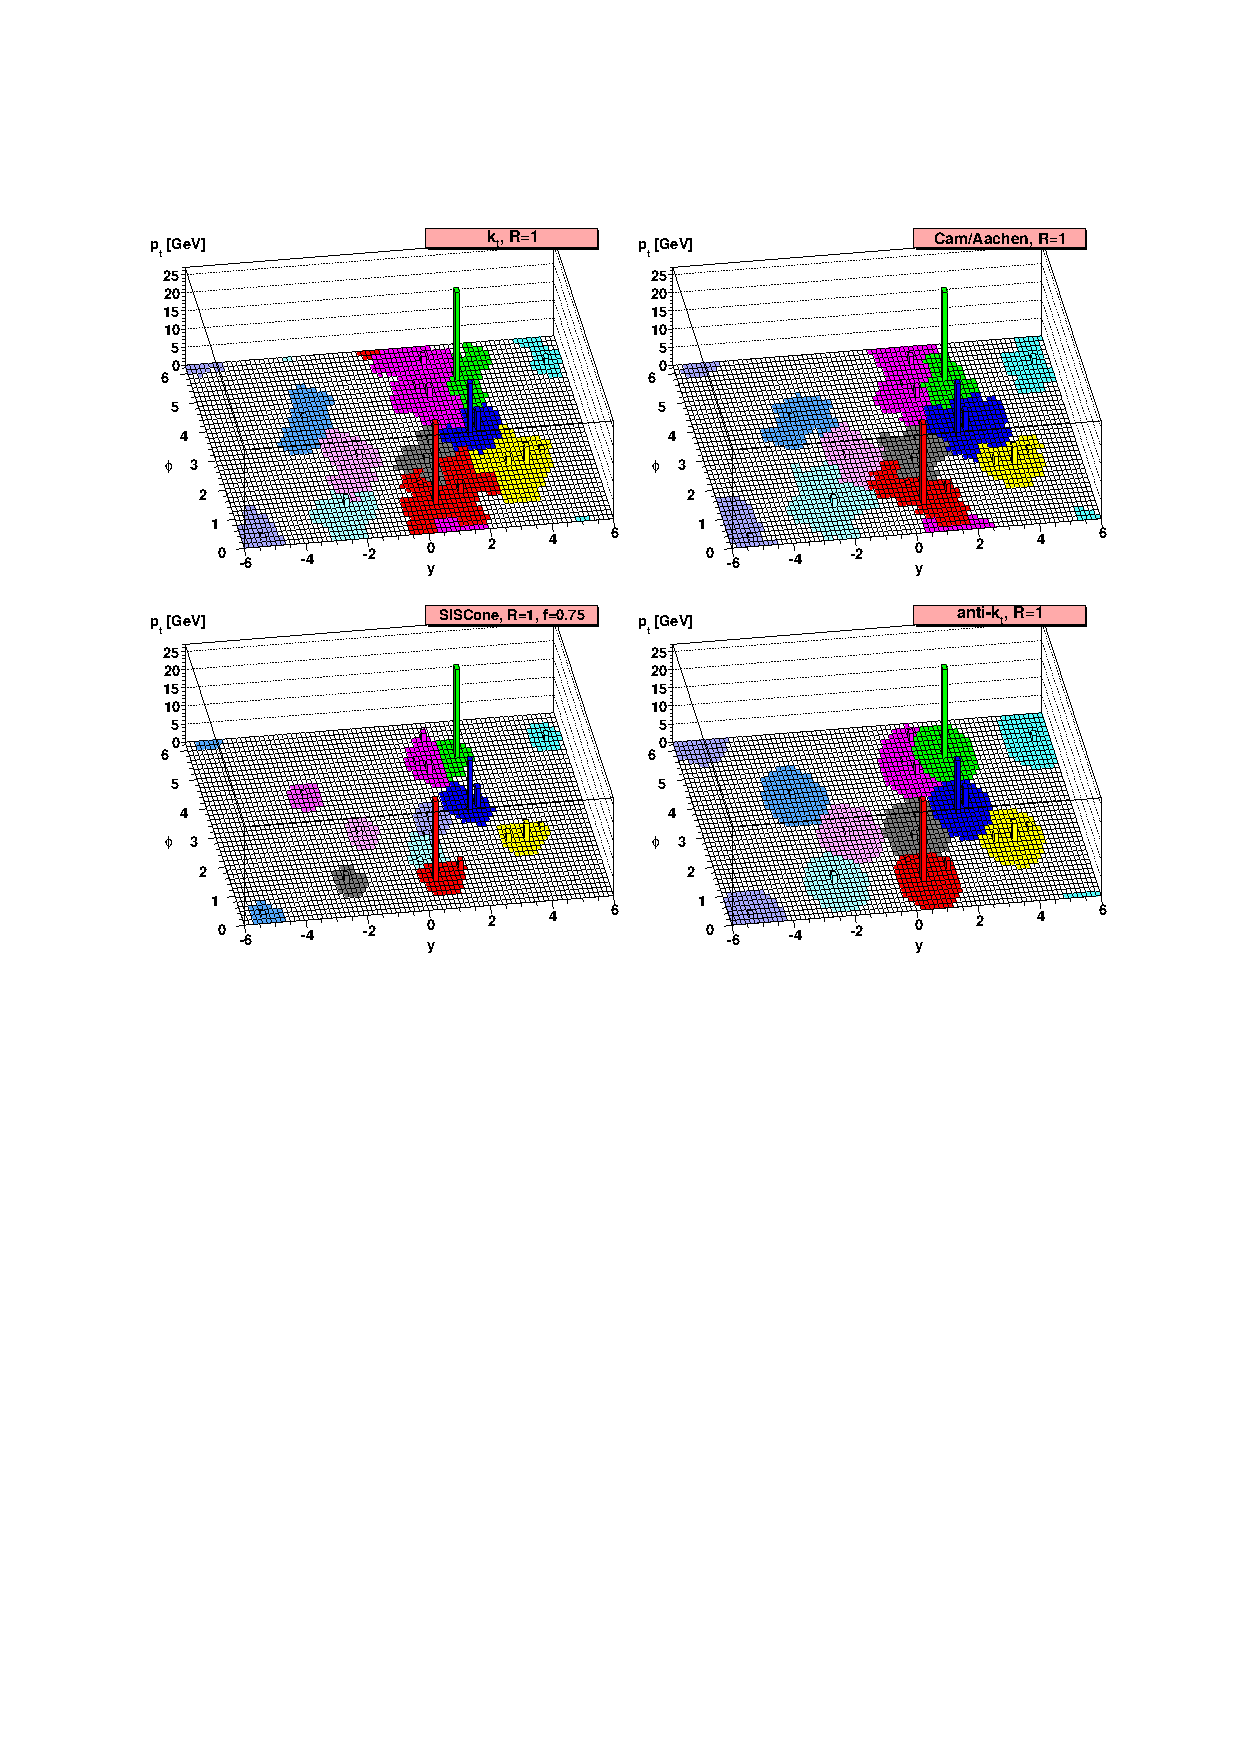
\includegraphics[width=1.2\textwidth]{/home/anter/Desktop/Thesis/Figures/cropped_JetAlgo.pdf}\\
\vspace*{4mm}
\caption[The clustering of particles into jets using different jet algorithms.]{The clustering of particles, in $y$-$\phi$ space at the parton level, into jets clustered with the \kt (top left), Cambridge/Aachen (top right), SISCone (bottom left) and anti-\kt (bottom right) algorithms with $R$ = 1. The towers represent the jet \pt. The anti-\kt algorithm gives circular jets while the jets produced with other three algorithms have irregular shapes. Taken from \cite{Salam:2009jx}.}
\label{fig:jet_algo}
\end{center}
\end{figure}

A jet algorithm must specify how to combine the momenta of different partons or particles going to be clustered into a jet. This is given by the recombination scheme. The most widely used recombination scheme is the $E$-scheme \cite{Blazey:2000qt} which corresponds to vector addition of four-momenta where the four-momenta of the jet is obtained by simply adding the four-momenta vector of merging particles.
 
The sequential clustering algorithms have always been favoured by theorists but not by experimentalists because of slow computational performance. However, the introduction of the \fastjet program \cite{Cacciari:2011ma} enhanced the speed of clustering algorithms and hence are preferred by experimentalists as well. This thesis studies the particles produced in proton-proton collisions by clustering them in to jets using anti-\kt algorithm with distance parameter $R$ = 0.7. These jets are observed in the Compact Muon Solenoid detector of the Large Hadron Collider, whose details are discussed in the coming chapter.

